\documentclass[
]{article}
\usepackage{xcolor}
\usepackage{amsmath,amssymb}
\usepackage{iftex}
\ifPDFTeX
  \usepackage[T1]{fontenc}
  \usepackage[utf8]{inputenc}
  \usepackage{textcomp}
\else
  \usepackage{unicode-math}
  \defaultfontfeatures{Scale=MatchLowercase}
  \defaultfontfeatures[\rmfamily]{Ligatures=TeX,Scale=1}
\fi
\usepackage{lmodern}
\ifPDFTeX\else
\fi
\usepackage{microtype}
\usepackage{longtable,booktabs,array}
\usepackage{graphicx}
\setlength{\emergencystretch}{3em}
\providecommand{\tightlist}{
  \setlength{\itemsep}{0pt}\setlength{\parskip}{0pt}}
\usepackage{bookmark}
\urlstyle{same}
\setcounter{secnumdepth}{3}
\setcounter{tocdepth}{3}
\usepackage{hyperref}
\usepackage{placeins}
\usepackage{float}
\title{\textbf{Computational Analysis of Newtonian vs Relativistic Gravitational Potentials: Error Quantification and Machine Learning Approximations}}
\hypersetup{
    colorlinks=true,
    linkcolor=blue,
    citecolor=blue,
    urlcolor=blue
}
\author{
Aayush Kumar\\
Independent Student Researcher\\
India\\
\href{mailto:aayushkumar_@outlook.com}{aayushkumar\_@outlook.com}
}
\date{25 June 2026}
\begin{document}
\maketitle
\section{Abstract}\label{abstract}
Understanding the applicability limits of classical gravitational models
and identifying the conditions under which relativistic corrections become
significant remain important challenges in computational physics. In this
study, a static relativistic gravitational potential is investigated
through an integrated framework combining analytical analysis, numerical
evaluation, and machine-learning-based approaches.

The relativistic formulation is analyzed and compared with the
corresponding Newtonian approximation through mathematical derivation
and computational error analysis. The deviation between the two models
is evaluated through relative error analysis, enabling a systematic
investigation of the transition between weak-field and strong-field
gravitational regimes.

To explore the capability of data-driven methods in approximating
nonlinear physical systems, a computational dataset is generated from
the analytical model and used to train multiple machine learning
algorithms. Linear regression, polynomial regression, neural networks,
and random forest regression are evaluated to compare their ability to
reproduce the behavior of the relativistic potential.

The results demonstrate that machine learning models can effectively
approximate the underlying physical relationship, with nonlinear
approaches providing significantly improved performance over simpler
regression methods. The predictions are interpreted as computational
approximations that complement the analytical formulation rather than
replacing the physical model.

This study presents a framework that combines theoretical physics,
numerical analysis, and machine learning for studying nonlinear
scientific systems. The approach highlights the potential of machine
learning as a tool for computational modeling while maintaining
consistency with established physical principles.

\noindent\textbf{Keywords:}
Gravitational potential;
Relativistic gravity;
Newtonian approximation;
Error analysis;
Schwarzschild spacetime;
Machine learning;
Random forest regression;
Computational physics

\tableofcontents
\newpage

\section{Introduction}\label{introduction}

\subsection{Motivation}\label{motivation}

Mathematical modeling provides a fundamental framework for describing
physical systems by establishing quantitative relationships between
observable quantities and theoretical predictions. Through appropriate
mathematical formulations, complex physical phenomena can be analyzed,
simulated, and compared under different conditions.

Gravitational systems represent an important example where the validity
and limitations of different theoretical descriptions must be carefully
examined. Newtonian gravity has successfully explained a wide range of
phenomena and remains highly accurate in weak gravitational fields.
However, its applicability becomes limited in regimes where spacetime
curvature and relativistic effects become significant
\cite{newton1687}. In such situations, general relativity provides the
appropriate theoretical framework for obtaining accurate descriptions of
gravitational behaviour \cite{einstein1916}.

Understanding the transition between classical and relativistic
descriptions is an important problem in computational physics because it
requires quantifying the deviation between different theoretical
models. Such analysis provides a systematic method for determining the
range of validity of classical approximations and identifying the
regimes where relativistic corrections become necessary.

In this study, this problem is investigated through a combined
analytical, numerical, and machine learning based approach. The aim is
not to modify the underlying physical formulation, but to examine how
computational techniques, including machine learning methods, can be
used as approximation tools for a theoretically defined gravitational
system.

\subsection{Background of Relativistic Potential
Models}\label{background-of-relativistic-potential-models}

The mathematical description of gravitational interactions has evolved
from classical formulations based on Newtonian mechanics to relativistic
models based on the geometry of spacetime
\cite{newton1687, einstein1916}. In Newtonian mechanics, gravitational
effects are represented through forces and associated potential
functions, which provide an effective description of the system under
appropriate assumptions.

The Newtonian potential provides an accurate approximation when the
gravitational field is sufficiently weak and spacetime curvature effects
can be neglected. However, as the strength of the gravitational field
increases, deviations from the classical approximation become
significant, requiring a relativistic description.

General relativistic models introduce corrections arising from the
interaction between matter, energy, and spacetime geometry
\cite{einstein1916}. Among the important solutions of Einstein's field
equations, the Schwarzschild solution provides a fundamental description
of the gravitational field produced by a static spherically symmetric
mass distribution \cite{schwarzschild1916}. The difference between
Newtonian and relativistic descriptions becomes increasingly important
near regions of strong gravitational fields.

Quantifying this difference provides insight into the applicability
limits of classical gravitational models. By evaluating the deviation
between the two descriptions, it becomes possible to determine the
regions where Newtonian approximations remain valid and where
relativistic corrections significantly influence the predicted
behaviour.

In this work, a static relativistic potential model is investigated using
analytical derivation and computational analysis
\cite{schwarzschild1916}. The corresponding Newtonian approximation is
examined, and the deviation between the two models is quantified through
error analysis. Furthermore, machine learning based approximations are
developed to investigate whether data-driven methods can effectively
reproduce the behaviour of the relativistic potential.

\subsection{Computational Physics and Machine
Learning}\label{computational-physics-and-machine-learning}

Computational methods have become an essential component of modern
scientific research because they allow physical systems to be explored
beyond the limitations of purely analytical approaches. Numerical
techniques enable systematic investigation of theoretical models,
parameter variations, and complex relationships between physical
quantities.

However, repeated evaluation of mathematical models can become
computationally demanding, particularly when large parameter spaces or
multiple simulations are involved. This has motivated the development of
alternative computational approaches capable of learning and
approximating complex relationships from generated or observed data.

Machine learning provides a framework for constructing predictive models
by identifying patterns within datasets. In scientific applications,
machine learning methods are increasingly used as surrogate models,
where computationally efficient approximations are developed while
maintaining consistency with established physical relationships
\cite{bishop2006, hastie2009}.

The application of machine learning in physics requires careful
validation against theoretical expectations because high predictive
accuracy alone does not guarantee physical reliability. Therefore, the
combination of analytical modelling, numerical analysis, and machine
learning evaluation provides a more complete approach for studying
scientific systems.

In this research, machine learning methods are applied to the static
relativistic potential model to investigate their ability to approximate
a known nonlinear physical relationship. The machine learning component
is considered as a complementary computational approach rather than a
replacement for the analytical formulation.

\subsection{Objectives and
Contributions}\label{objectives-and-contributions}

The primary objective of this study is to develop a computational
framework that integrates theoretical gravitational modelling, numerical
error analysis, and machine learning based approximation for analysing a
static relativistic potential system.

The study focuses on understanding the relationship between the
relativistic and Newtonian descriptions of gravitational behaviour and
evaluating whether machine learning models can accurately reproduce the
resulting nonlinear relationship.

The major objectives of this research are:

\begin{enumerate}
\def\labelenumi{\arabic{enumi}.}
\item
  Developing the mathematical formulation of the static relativistic
  potential and its corresponding Newtonian approximation.
\item
  Quantifying the deviation between the relativistic and classical
  models using analytical and numerical error analysis.
\item
  Investigating the transition between strong-field and weak-field
  regimes through the behaviour of the relative error.
\item
  Constructing a computational dataset generated from the theoretical
  model for machine learning experiments.
\item
  Evaluating multiple machine learning architectures, including
  regression models, neural networks, and ensemble-based methods.
\item
  Comparing model performance using standard regression evaluation
  metrics and analysing their ability to approximate the physical
  relationship.
\end{enumerate}

The main contribution of this work is the integration of three
complementary components: analytical gravitational modelling, numerical
quantification of model deviation, and machine learning based
approximation. Rather than considering artificial intelligence as an
alternative to theoretical physics, this study investigates its role as
a computational tool for representing known physical relationships.

\subsection{Organization of the Paper}\label{organization-of-the-paper}

The remainder of this paper is organized as follows. Section 2 presents
the theoretical framework of the static relativistic potential and its
Newtonian approximation. Section 3 describes the mathematical
formulation and derivation of the error function. Section 4 presents the
numerical analysis of the relativistic and classical models. Section 5
discusses computational implementation and dataset generation. Section 7
introduces the machine learning framework and describes the evaluated
models. Section 8 presents the model performance results and analysis.
Finally, Section 9 discusses the physical interpretation, limitations,
and future extensions of the study.

\section{Theoretical Framework}\label{theoretical-framework}

\subsection{Physical Motivation}\label{physical-motivation}

Mathematical models describing physical systems need to be accurate and
reflect correctly the physical phenomena occurring within such systems
depending on various conditions. While classical gravitational systems
give reliable predictions in many cases, their limitations arise when
dealing with strong enough gravitational fields and relativistic
effects.

Comparison of different descriptions gives insight into the boundaries
of applicability of one or another physical model. The comparison of the
deviation between such models enables us to quantify the transition from
one regime to another.

In the case of the weak-field approximation, the Newtonian approximation
gives a good description, while relativistic corrections can be
neglected. As the characteristic distance from the gravitational field
decreases, relativistic corrections start to play a bigger role and the
classical description becomes less precise.

The aim of this study is to examine the process of the transition from
the classical to the relativistic description by constructing a
computational framework which allows us to compare the relativistic and
the Newtonian potentials.

By integrating analytical methods, numerical simulations, and machine
learning algorithms, this study investigates both the underlying
physical behaviour of the system and the feasibility of developing
accurate computational approximations.

The theoretical framework proposed in this section serves as a basis for
the subsequent mathematical description, analysis of errors and machine
learning experiments.

\subsection{Dimensionless Representation}\label{dimensionless-representation}

In order to facilitate the mathematical manipulation of the model and
generalize the outcome to various physical scales, the gravitational
field is expressed in terms of a dimensionless variable.

The normalization of the radius vector is done using the characteristic
length of the relativistic gravitational system:

\[
x=\frac{r}{r_s}
\]

where:
\begin{itemize}
\item $r$ represents the radial distance from the gravitational source.
\item $r_s$ represents the characteristic relativistic scale of the system.
\item $x$ represents the normalized dimensionless radial parameter.
\end{itemize}

Dimensional variable gives several benefits. First, it eliminates
dependence on the specific physical units and allows the system to be
studied in terms of the relative distance instead of the absolute one.

The variable (x) can be also used for the examination of various
gravitational regimes. The values of the variable (x) that are close to
the characteristic length correspond to the relativistic gravitational
systems. Larger values of the variable (x) correspond to gravitational
systems with low intensity where classical approximation is a better
choice.

In terms of this normalized distance both the relativistic and Newtonian
potential models can be expressed, and thus the comparison between them
will not depend on any specific physical system but will rely only on
mathematics.

This dimensionless formulation forms the basis for the analytical
derivations and computational simulations performed in the following
sections.

\subsection{Newtonian Approximation}\label{newtonian-approximation}

The Newtonian gravitational potential provides the classical reference
model for gravitational interactions in the weak-field limit. In this
work, it is used as the baseline model against which the relativistic
correction is quantified.

The Newtonian approximation assumes a fixed space-time framework and is
accurate when gravitational fields are sufficiently weak. However, near
strong-field regions, deviations from the Newtonian description become
significant, motivating comparison with a relativistic formulation.

The mathematical definition and normalization of the Newtonian potential
used in this study are presented in Section~\ref{newtonian-potential-equation}.

\subsection{Static Relativistic Potential Model}

To incorporate strong-field gravitational effects, this study considers a
static relativistic potential derived from the Schwarzschild solution of
general relativity.

Unlike the Newtonian approximation, the relativistic model introduces
nonlinear corrections arising from spacetime curvature. These corrections
become increasingly important near the Schwarzschild radius.

The complete mathematical formulation, normalization procedure, and
dimensionless representation of the relativistic potential are described
in Section~\ref{relativistic-potential-equation}.

\subsection{Relativistic-Newtonian Comparison}\label{relativisticnewtonian-comparison}

The Newtonian and relativistic potential models describe the same
gravitational system but differ in their treatment of gravitational
effects.

The Newtonian potential provides a classical approximation that assumes
weak gravitational fields and neglects relativistic corrections. In
contrast, the relativistic potential incorporates nonlinear effects that
arise from the relativistic description of gravity.

A comparison of the two models allows the accuracy of the classical
approximation to be evaluated as a function of the normalized radial
coordinate. In regions far from the characteristic relativistic scale,
the two potentials exhibit similar functional behavior, allowing
Newtonian gravity to provide a qualitative approximation. However,
quantitative comparison through relative error analysis is required to
determine the accuracy of this approximation.

Closer to the strong-field region, however, the difference between the
models becomes increasingly significant. This deviation reflects the
growing importance of relativistic corrections and motivates the use of
quantitative error analysis.

To measure the discrepancy between the two descriptions, a relative
error function is introduced in the following section. This function
provides a numerical basis for evaluating the validity range of the
Newtonian approximation and identifying the transition between classical
and relativistic gravitational behavior.

\section{Mathematical Formulation}\label{mathematical-formulation}

\subsection{Relativistic Potential Equation}\label{relativistic-potential-equation}

The relativistic gravitational potential investigated in this study is
derived from the Schwarzschild solution and is expressed as

\[
\Phi_{GR}(r)=
\frac{c^2}{2}
\left(
\sqrt{1-\frac{2GM}{rc^2}}
-1
\right).
\]

where:
\begin{itemize}
\item $G$ represents the gravitational constant.
\item $M$ represents the mass of the gravitating source.
\item $r$ represents the radial distance.
\item $c$ represents the speed of light.
\end{itemize}

Introducing the Schwarzschild radius

\[
r_s=\frac{2GM}{c^2}
\]

and the dimensionless coordinate about which we discussed in Section~\ref{dimensionless-representation}.

\[
x=\frac{r}{r_s},
\]

Substituting:

\[
GM=\frac{r_sc^2}{2}
\]

and

\[
r=xr_s,
\]

we obtain:

\[
\Phi_{GR}(x)=
\frac{c^2}{2}\left(\sqrt{1-\frac{1}{x}}-1\right).
\]

the dimensionless Relativistic potential is obtained by normalizing with
$c^2$:

\[
\phi_{GR}(x)
=
\frac{\Phi_{GR}}{c^2}
=
\frac{1}{2}
\left(
\sqrt{1-\frac{1}{x}}
-1
\right)
\]

\textbf{This equation represents the reference relativistic model used
throughout the study.} The nonlinear square-root dependence introduces
deviations from classical gravity that become significant near the
Schwarzschild radius.

For large values of (x), the relativistic potential follows the same
inverse-distance dependence as the Newtonian approximation. However,
because the leading-order coefficients differ, the two potentials do not
converge to the same normalized value. The difference arises because the adopted relativistic potential is normalized through the Schwarzschild metric expression rather than constructed as the classical Newtonian limit; therefore the comparison is performed within the defined potential formulation. This difference is quantified
through the relative error analysis performed in later
sections. Therefore, the weak-field limit in this formulation should be
interpreted as convergence in functional behavior rather than exact
numerical agreement between the two normalized potentials.

\subsection{Newtonian Potential Equation}\label{newtonian-potential-equation}

Newtonian Potential Equation The Newtonian gravitational potential is
taken as the classical reference potential for comparison purposes with
the relativistic potential equation. The potential equation represents
the gravitational effect of the mass source assuming that the effects of
spacetime and the gravitational field are in the weak-field
approximation region.

The standard Newtonian gravitational potential is given by:

\[\Phi_N(r)=-\frac{GM}{r}\]

where:
\begin{itemize}
\item $G$ represents the gravitational constant.
\item $M$ represents the mass of the gravitational source.
\item $r$ represents the radial distance from the source.
\end{itemize}

Using the dimensionless radial coordinate introduced previously in Section~\ref{dimensionless-representation}:

\[x=\frac{r}{r_s}\]

and the Schwarzschild radius

\[
r_s=\frac{2GM}{c^2}
\]

the normalized Newtonian potential becomes:

\[
\phi_N(x)=
\frac{\Phi_N}{c^2}
=
-\frac{GM}{rc^2}
\]

Substituting:

\[
GM=\frac{r_sc^2}{2}
\]

and

\[
r=xr_s,
\]

we obtain:

\[
\phi_N(x)=-\frac{1}{2x}
\]

\textbf{This normalized expression provides a simplified representation that
allows direct comparison with the relativistic potential model.} 

The Newtonian approximation serves as the standard for which the
relativistic corrections are taken into consideration. For large values
of (x), both models exhibit similar inverse-distance behavior. However,
the relative error analysis is required to determine the actual
quantitative agreement between the two descriptions. However, as (x)
goes deeper into stronger-field regions, the relativistic potential
starts to differ from the classical approximation.

\subsection{Derivation of Relative Error Expression}\label{derivation-of-relative-error-expression}

To quantify the difference between the relativistic and Newtonian
descriptions, the relative error between the two potential models is
calculated.

The relative error provides a measure of how much the Newtonian
approximation deviates from the relativistic potential at a given value
of the normalized radial coordinate (x).

The general form of the relative error is defined as:

\[
\epsilon(x)=
\left|
\frac{\phi_{GR}(x)-\phi_N(x)}
{\phi_{GR}(x)}
\right|
\times 100
\]

where:
\begin{itemize}
\tightlist
\item
  $\phi_{GR}(x)$ represents the normalized relativistic potential,
\item
  $\phi_{N}(x)$ represents the normalized Newtonian approximation,
\item
  $\epsilon(x)$ represents the percentage deviation between the two
  models.
\end{itemize}

Substituting the expressions for the relativistic and Newtonian
potentials into the error equation gives a mathematical relationship
describing the accuracy of the classical approximation across different
gravitational regimes.

This error function allows the transition between relativistic and
classical behavior to be studied quantitatively. When $\epsilon(x)$ is
small, the Newtonian model provides a close approximation to the
relativistic system. However, an increasing value of $\epsilon(x)$
indicates that relativistic corrections become significant.

The resulting error function is evaluated computationally over a range
of (x) values to analyze the behavior of the approximation and identify
regions where classical gravity remains sufficiently accurate.

This formulation provides the connection between the theoretical model
and the numerical analysis performed in this study.

\subsection{Simplified Error Formula}\label{simplified-error-formula}

After substituting the relativistic and Newtonian potential expressions
into the relative error equation, the resulting expression can be
simplified to obtain a direct relationship between the error and the
normalized radial coordinate (x).

The simplified form obtained is:

\[
\epsilon(x)=
100
\left|\frac{
-x^{3/2}+\sqrt{x}+x\sqrt{x-1}
}
{
x(-\sqrt{x}+\sqrt{x-1})
}\right|
\]

This expression represents the percentage deviation between the
relativistic potential and the Newtonian approximation as a function of
the dimensionless radial coordinate.

The equation provides a direct way to analyze how the accuracy of the
Newtonian model changes across different gravitational regimes. As (x)
increases, the relativistic corrections become smaller and the error
approaches the weak-field limit, where the Newtonian approximation
becomes increasingly accurate.

Conversely, for values of (x) closer to the strong-field region, the
deviation between the two models becomes more significant. This behavior
reflects the increasing influence of relativistic effects as the system
moves away from the conditions where classical gravity provides a
reliable approximation.

The simplified error expression is particularly useful because it
removes the need to repeatedly compare the two potential functions
separately. Instead, the accuracy of the Newtonian approximation can be
directly evaluated from a single mathematical relationship.

This analytical formulation is later used for numerical error analysis,
including the determination of accuracy thresholds and the
identification of the transition region between relativistic and
classical gravitational behavior.

\section{Error Analysis}\label{error-analysis}

\subsection{Error Behaviour}\label{error-behaviour}

The relative error function derived in the previous section provides a
quantitative measure of the difference between the relativistic
potential and the Newtonian approximation. By evaluating this function
over a range of values of the normalized radial coordinate (x), the
accuracy of the classical model can be studied.

The behavior of the error is expected to depend strongly on the
gravitational regime being considered. In regions closer to the
characteristic relativistic scale, the effects of relativistic
corrections become more significant, resulting in a larger deviation
between the two potential models.

As the value of (x) increases, the gravitational field becomes weaker
and the functional behavior of the relativistic and Newtonian
descriptions becomes increasingly similar. However, due to the
difference in their asymptotic normalization, the relative error does
not decrease to zero and instead approaches a limiting value.

The variation of the relative error with respect to the normalized
radial coordinate is shown in Figure 1.

\begin{figure}[H]
\centering
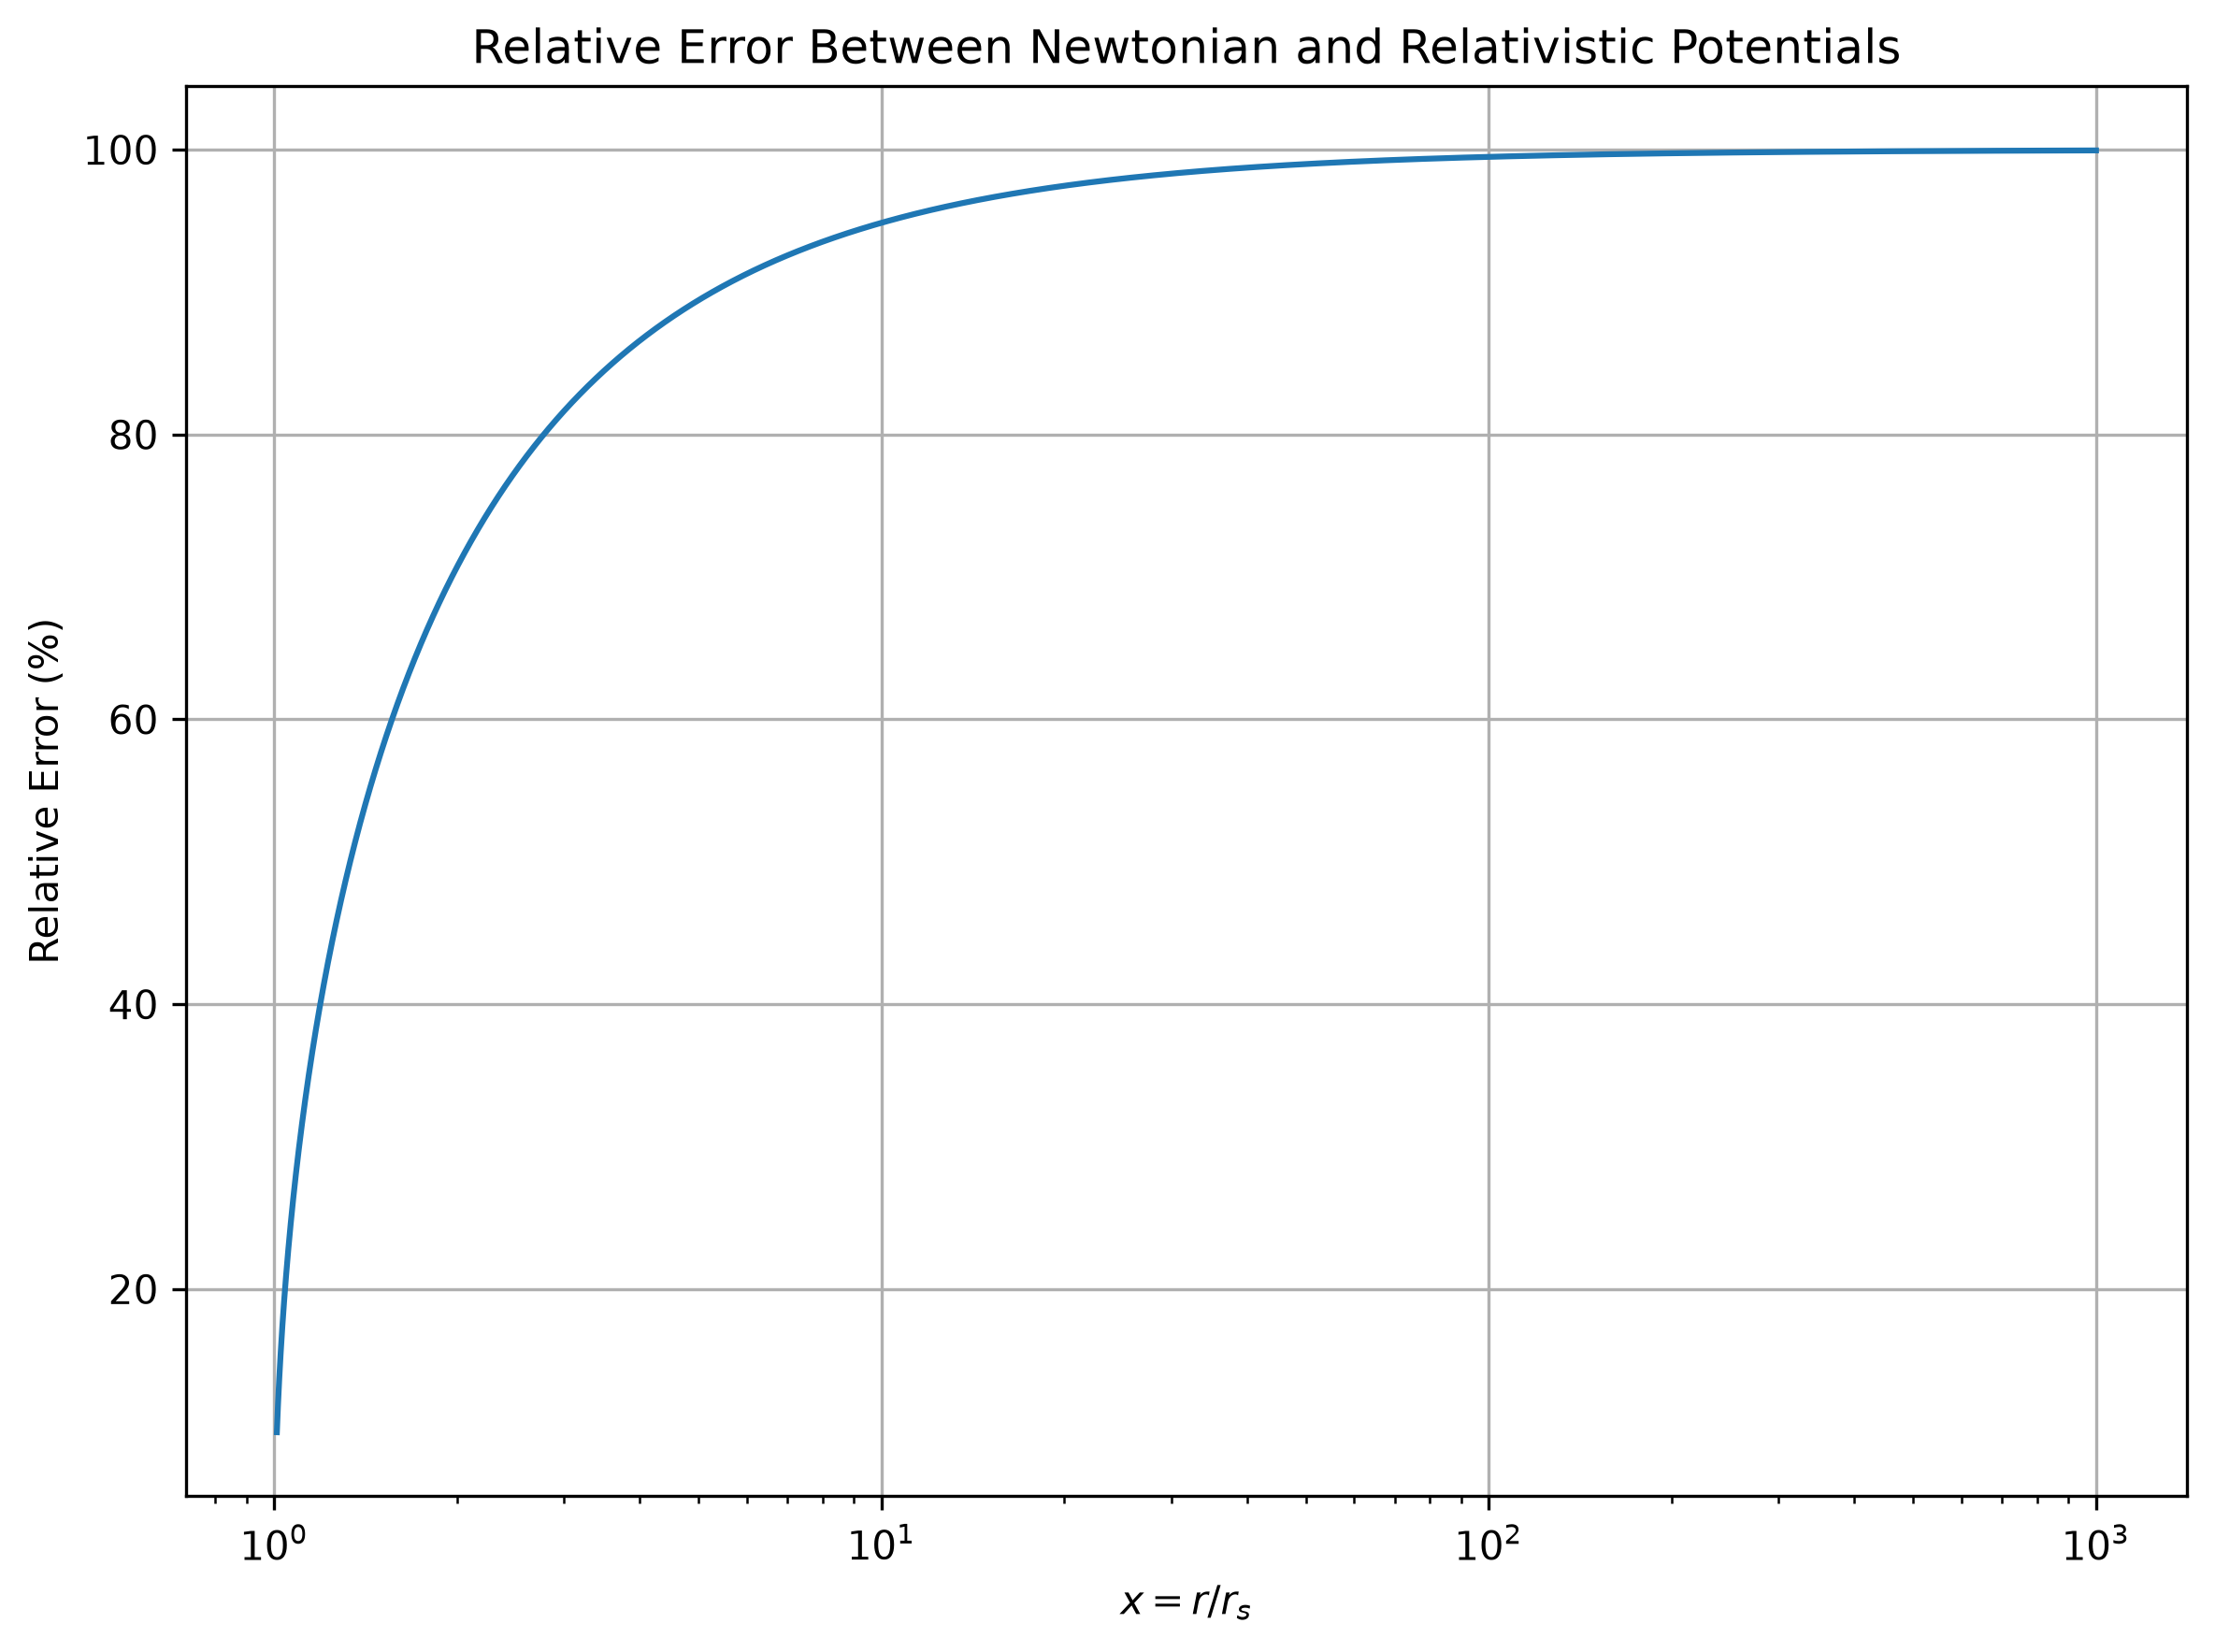
\includegraphics[width = 0.85\textwidth]{../04_Graphs_and_Figures/relative_error_plot.png}
\caption{Relative error between the normalized relativistic potential and the Newtonian approximation as a function of the dimensionless radial coordinate $x$. The minimum error occurs near $x=1.01$, while the error increases toward the weak-field regime due to the differing asymptotic normalizations of the two models.}
\label{fig:relative_error_plot}
\end{figure}

This behavior demonstrates the transition from a region where
relativistic corrections significantly modify the potential toward a
region where both models exhibit similar qualitative inverse-distance
behavior. However, due to the difference in asymptotic normalization,
the Newtonian model does not achieve vanishing relative error under the
chosen formulation.

The numerical evaluation of the error function allows this transition to
be examined quantitatively rather than only through theoretical
assumptions. By measuring how the error changes with (x), the range in
which Newtonian gravity achieves a specified accuracy can be determined.

The error analysis therefore provides an important link between the
theoretical formulation and the quantitative evaluation of the classical
approximation within the considered model.

\subsection{Error Threshold Analysis}\label{error-threshold-analysis}

A numerical threshold analysis was performed to determine whether the
Newtonian approximation reaches commonly used accuracy levels within the
sampled domain.

The threshold condition was defined as:

\[
\epsilon(x)\leq \epsilon_{limit}
\]

where $\epsilon_{limit}$ represents a specified maximum relative
error.

Three thresholds were investigated:

\begin{itemize}
\tightlist
\item
  10\% relative error,
\item
  5\% relative error,
\item
  1\% relative error.
\end{itemize}

The numerical evaluation showed that the relative error reaches its
minimum value near the lower boundary of the investigated domain:

\[
x = 1.01
\]

with a corresponding relative error of approximately:

\[
\epsilon = 9.950372%
\]

However, the analysis further revealed that the relative error never
falls below either the 5\% or 1\% thresholds within the investigated
domain:

\[
1.01 \le x \le 1000
\]

The minimum observed relative error across the sampled dataset was
approximately 9.95\%.

These results indicate that, for the specific relativistic potential
considered in this study, the Newtonian approximation does not achieve
better than approximately 10\% accuracy within the investigated domain.
The minimum relative error occurs near the lower boundary of the sampled
range (x = 1.01), while the discrepancy increases as x becomes larger.

This behavior arises from the different asymptotic forms of the two
potentials. In the large-distance limit, the relativistic potential
approaches $\phi_{GR} \approx -1/(4x)$, whereas the Newtonian approximation follows
$\phi_{N} = -1/(2x)$. Consequently, the relative error increases toward $100\%$
as $x \to \infty$ rather than remaining near $10\%$. Therefore, the observed $9.95\%$
value represents the minimum error within the chosen domain, not the
asymptotic error behavior.

\subsection{Strong-Field and Weak-Field Transition}\label{strong-field-and-weak-field-transition}

The variation of the relative error with the normalized radial
coordinate provides a way to identify the transition between
strong-field and weak-field gravitational regimes.

In the strong-field region, where (x) approaches the characteristic
relativistic scale, the assumptions behind the Newtonian approximation
become less accurate. The contribution of relativistic corrections
becomes more significant, leading to a larger difference between the
relativistic and classical potential models.

As the value of (x) increases, the influence of relativistic corrections
gradually decreases. The system moves toward the weak-field regime,
where the Newtonian approximation becomes increasingly consistent with
the relativistic description.

This transition can be understood through the behavior of the relative
error. A larger error indicates that the classical approximation does
not fully capture the physical behavior of the system, while a smaller
error indicates that the Newtonian model provides an effective
approximation.

By analyzing the points where the error crosses predefined accuracy
limits, the boundary between these regimes can be estimated
quantitatively. Instead of defining the transition only through
theoretical assumptions, this approach provides a measurable criterion
based on the accuracy of the approximation.

The identification of this transition region is important because it
establishes the range in which classical gravitational models remain
applicable and the range where relativistic corrections become
necessary. This analysis also provides a physically meaningful
interpretation of the dataset later used for machine learning
experiments.

\subsection{Asymptotic Behaviour}\label{asymptotic-behaviour}

The asymptotic behavior of the relativistic and Newtonian potentials
provides important insight into their relationship in the weak-field
regime.

As the normalized radial coordinate (x) increases, both potentials
approach an inverse-distance dependence, indicating similar qualitative
behavior. However, they do not converge to the same value because their
leading-order terms differ:

\[
\phi_{GR}\approx-\frac{1}{4x}
\]

whereas

\[
\phi_N=-\frac{1}{2x}.
\]

Therefore, the Newtonian approximation captures the general
distance-dependent trend of the relativistic potential but retains a
systematic quantitative discrepancy due to the difference in
normalization.
The observed asymptotic discrepancy is a consequence of the chosen
normalization of the relativistic potential and should not be interpreted
as a failure of the Newtonian weak-field approximation itself.

Numerical evaluation of the relative error reveals that the minimum
observed deviation within the investigated domain occurs near the lower
boundary:

\[
\epsilon_{min}=9.950372\%
\]

at approximately:

\[
x=1.01.
\]

The difference between the relativistic and Newtonian potentials is
shown in Figure 2, illustrating the systematic deviation between the two
models.

\begin{figure}[H]
\centering
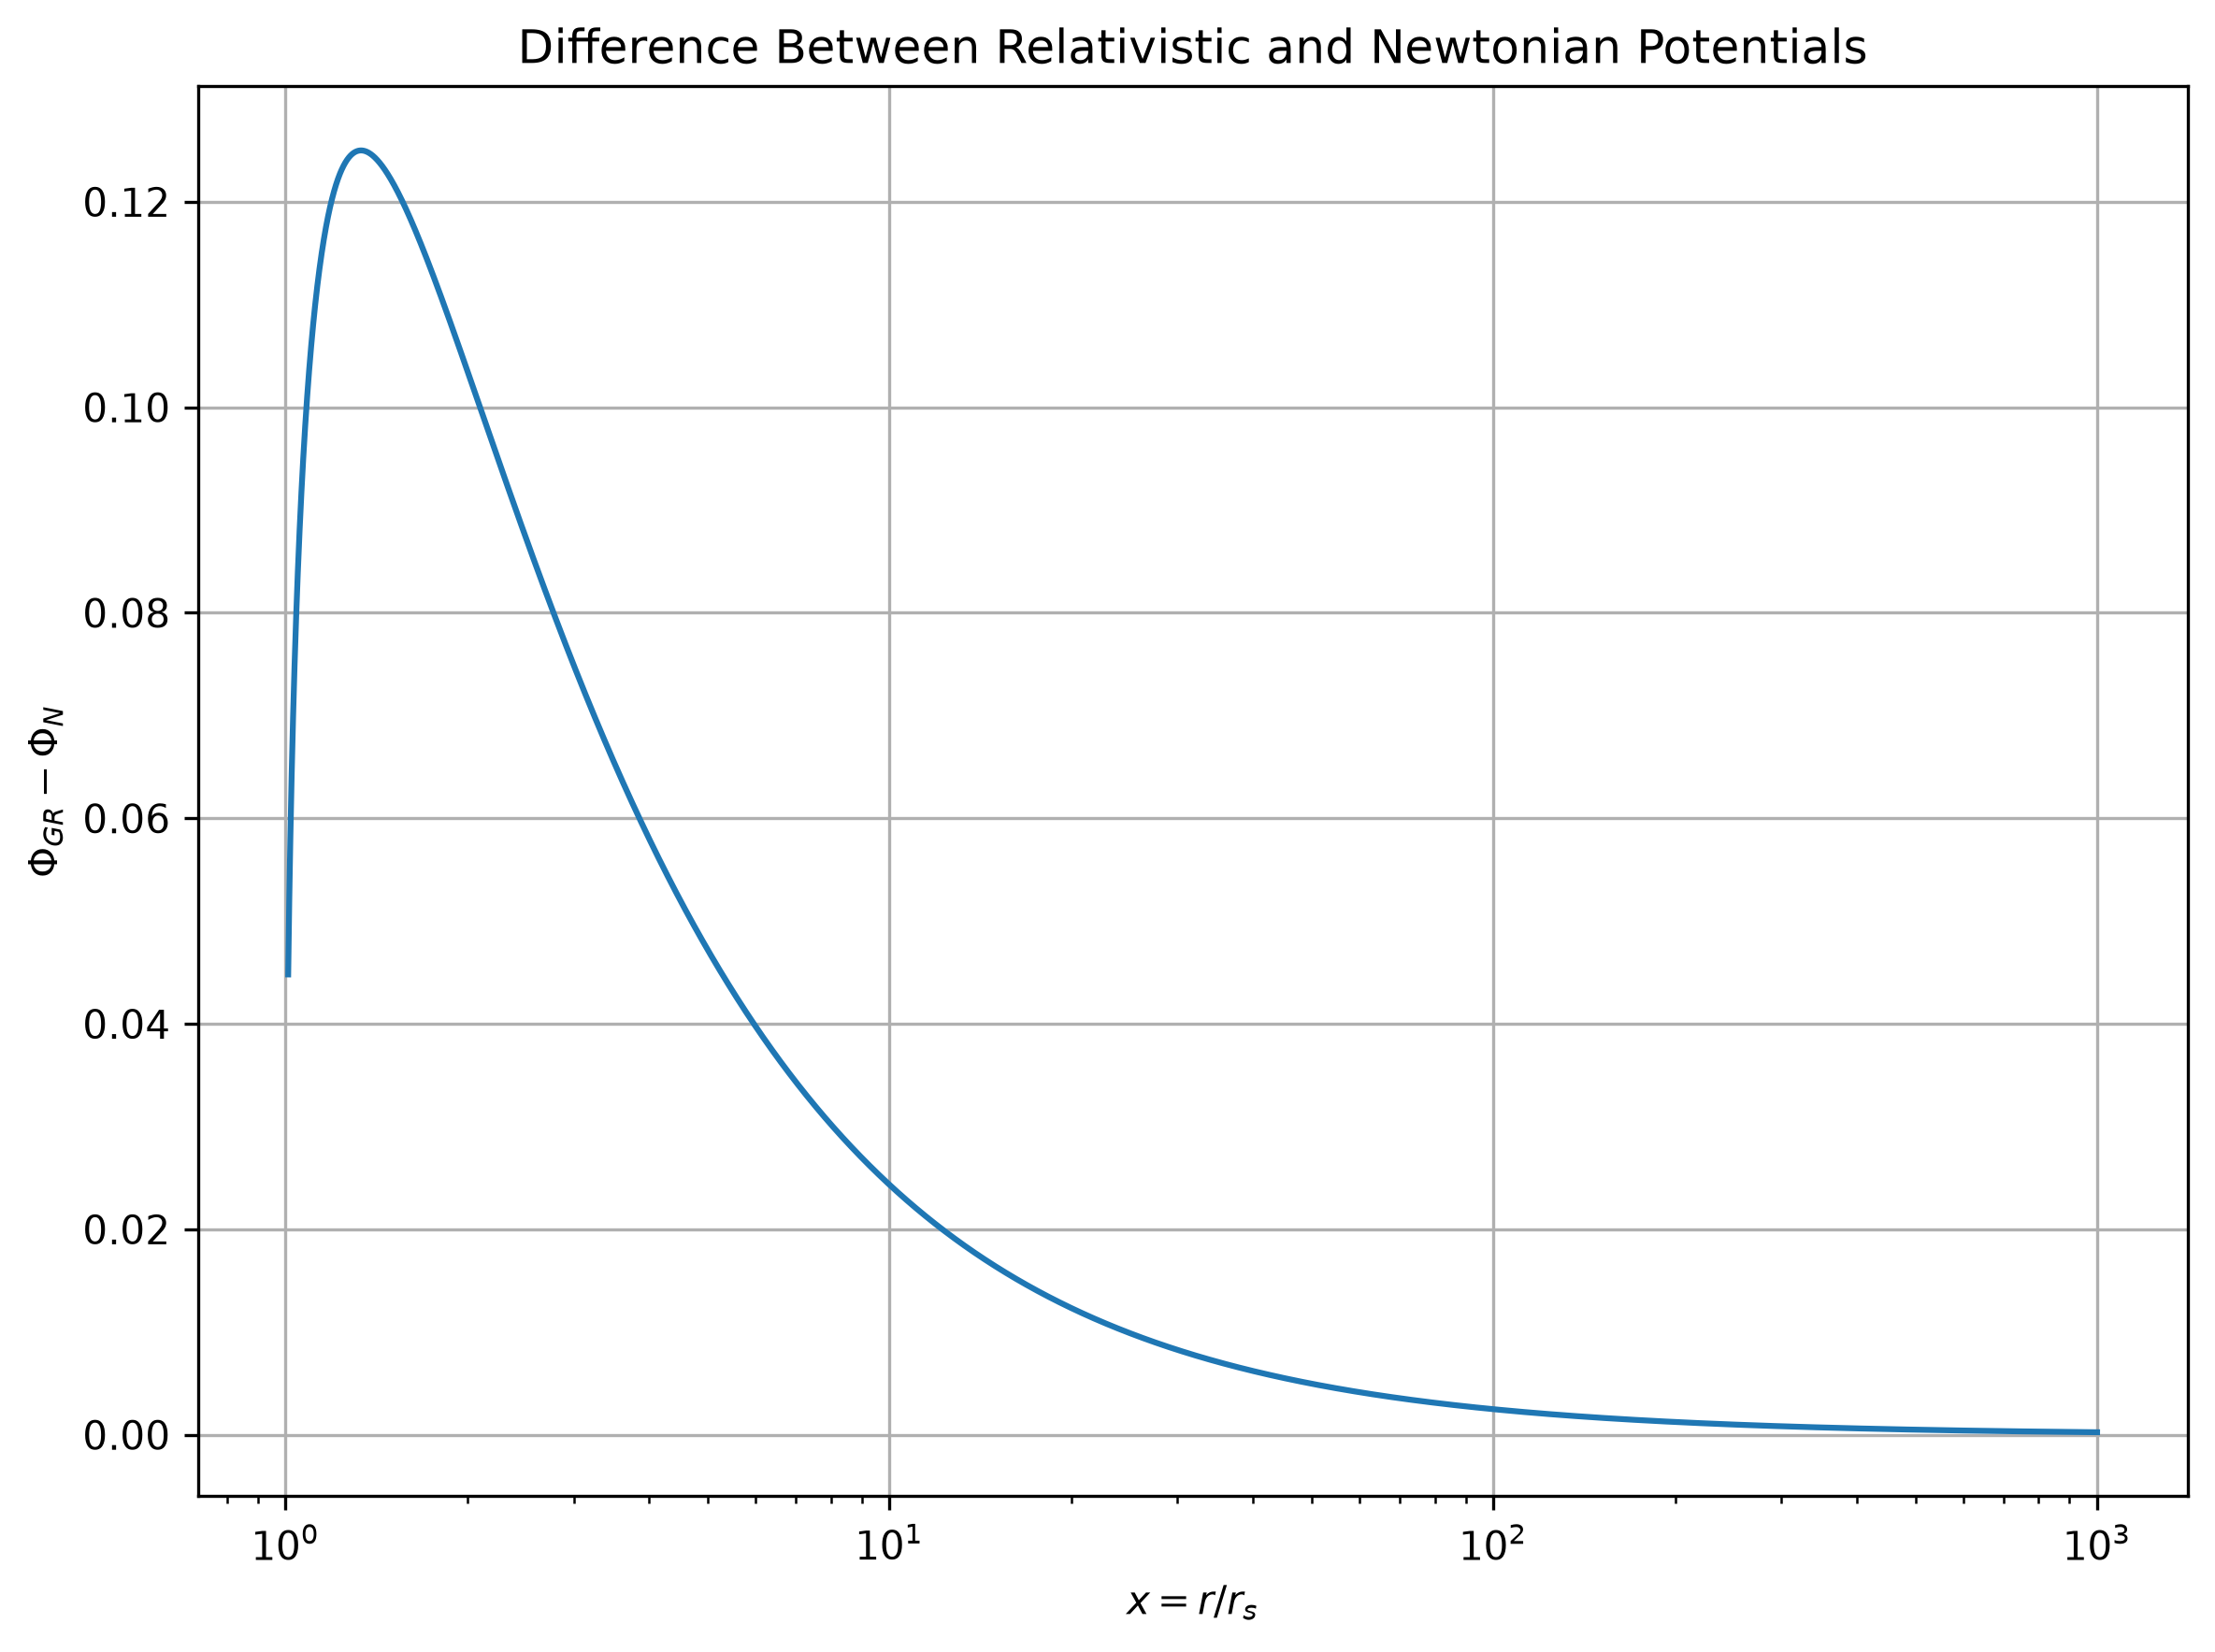
\includegraphics[width=0.85\textwidth]{../04_Graphs_and_Figures/difference_plot.png}
\caption{Difference $\Delta\phi=\phi_{GR}-\phi_N$ between the normalized relativistic and Newtonian potential models across the investigated domain. The plot illustrates the systematic deviation between the two formulations.}
\label{fig:difference_plot}
\end{figure}

However, this minimum value should not be interpreted as the asymptotic
error. As x increases, the relative error grows and approaches 100\% in
the large-distance limit because the ratio between the leading-order
terms remains different.

This behavior explains why the 5\% and 1\% accuracy thresholds are never
reached within the sampled range:

\[
1.01 \le x \le 1000.
\]

The location of the maximum deviation is further illustrated in Figure
3.

\begin{figure}[H]
\centering
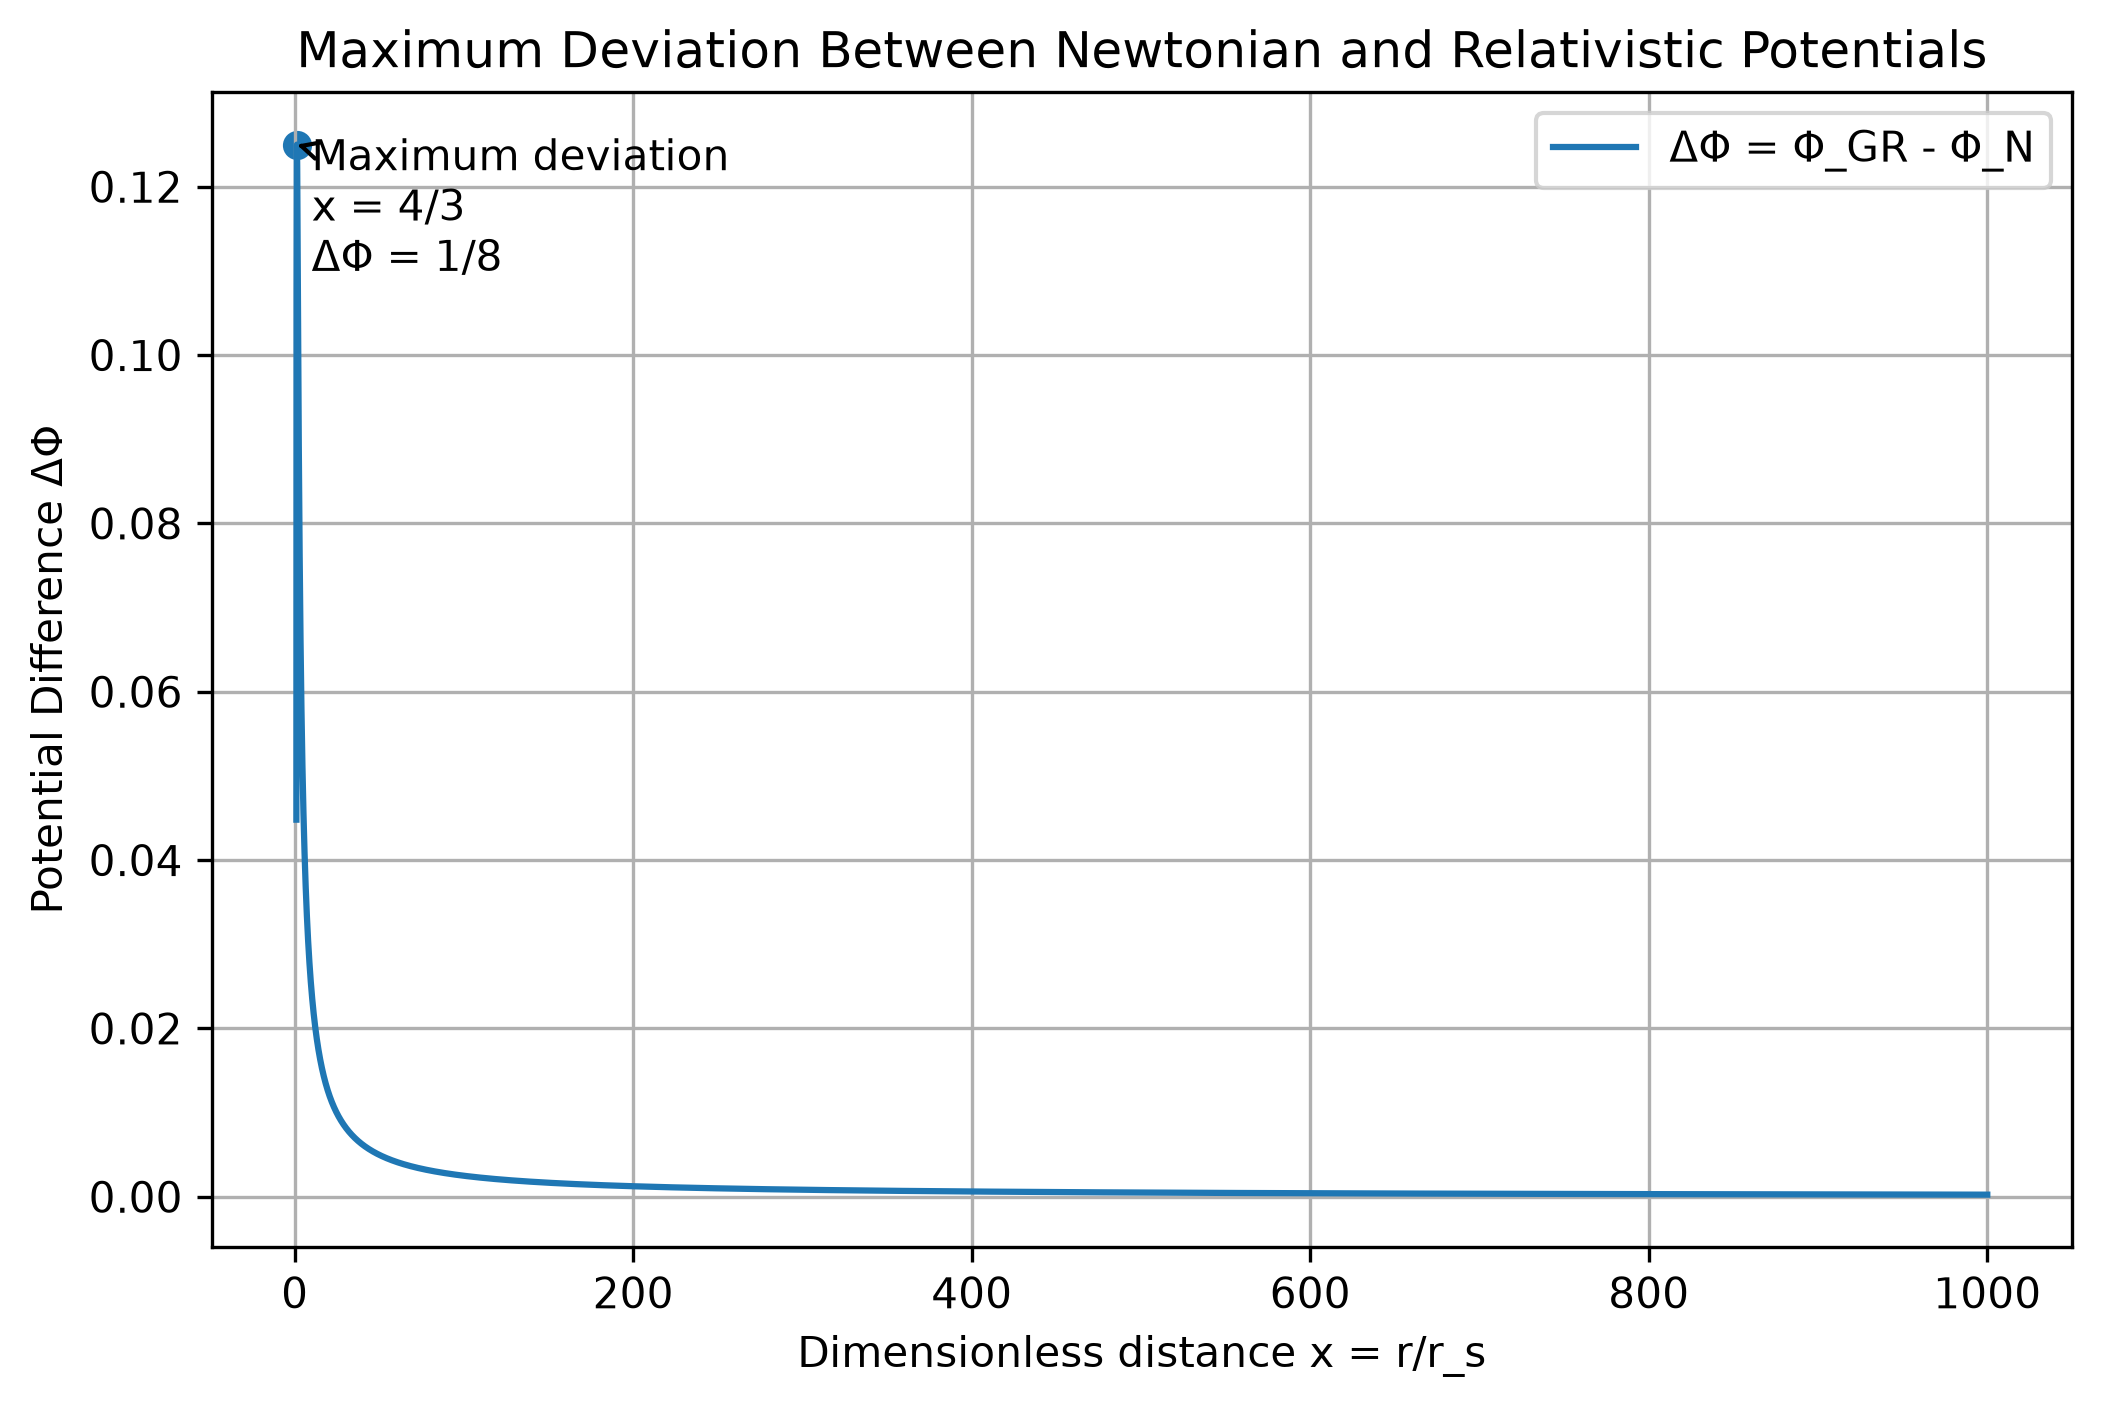
\includegraphics[width=0.85\textwidth]{../04_Graphs_and_Figures/annotated_difference_plot.png}
\caption{Annotated plot of the potential difference showing the location of maximum deviation between the relativistic and Newtonian models.}
\label{fig:annotated_difference_plot}
\end{figure}

Therefore, while the Newtonian approximation reproduces the qualitative
inverse-distance behavior of the relativistic potential, explicit error
analysis reveals a persistent and increasing quantitative discrepancy.
This result demonstrates the importance of evaluating approximation
accuracy through numerical comparison rather than assuming convergence
solely from similar functional behavior.

\section{Gravitational Field Analysis}\label{gravitational-field-analysis}

\subsection{Newtonian Field}\label{newtonian-field}

The gravitational field is obtained from the spatial variation of the
potential. In the Newtonian framework, the gravitational field is
defined as the negative gradient of the gravitational potential:

\[
g_N=-\frac{d\Phi_N}{dr}
\]

Using the Newtonian potential:

\[
\Phi_N(r)=-\frac{GM}{r}
\]

the corresponding gravitational field becomes:

\[
g_N=\frac{GM}{r^2}
\]

This represents the classical inverse-square behavior of gravity, where
the field strength decreases with increasing distance from the source.

Using the normalized coordinate (x), the Newtonian field can be analyzed
in terms of the relative distance scale rather than absolute units. This
allows direct comparison with the relativistic field representation.

The Newtonian field provides the classical reference behavior for
evaluating the influence of relativistic corrections. In the weak-field
regime, it is expected to closely match the relativistic prediction,
while deviations become more noticeable as the system approaches
stronger gravitational regions.

The analysis of the Newtonian field therefore provides the baseline
required for understanding how relativistic effects modify the
gravitational behavior of the system.

\subsection{Relativistic Field}\label{relativistic-field}

In the relativistic description, the gravitational field is obtained
from the variation of the relativistic potential with respect to the
radial coordinate:

\[
g_{GR}=-\frac{d\Phi_{GR}}{dr}
\]

Unlike the Newtonian formulation, the relativistic field includes
corrections that arise from the modified structure of the gravitational
potential. These corrections become increasingly important in regions
where the gravitational field is stronger.

The behavior of the relativistic field differs from the Newtonian
prediction mainly due to the nonlinear dependence introduced by the
relativistic formulation. At larger values of (x), where the
gravitational field is weaker, the relativistic field gradually
approaches the Newtonian result. However, closer to the strong-field
region, the difference between the two descriptions becomes more
significant.

The comparison of these two field models provides additional information
beyond the potential analysis. While the potential comparison measures
the difference in gravitational energy representation, the field
comparison examines how the gravitational influence itself changes
across different regimes.

This analysis helps establish a more complete understanding of the
system by considering both the potential and the resulting field
behavior before applying computational and machine learning methods.

\subsection{Comparative Analysis}\label{comparative-analysis}

The comparison between the Newtonian and relativistic gravitational
fields provides a broader perspective on the transition between
classical and relativistic descriptions.

In the weak-field regime, the difference between the two models becomes
minimal, indicating that Newtonian gravity provides an accurate
approximation of the relativistic behavior. This agreement explains why
classical gravitational models remain effective for many practical
applications where relativistic corrections are extremely small.

However, as the system moves toward stronger gravitational regions, the
relativistic corrections become increasingly important. The deviation
between the two field descriptions reflects the limitations of the
classical approximation and highlights the need for a relativistic
treatment.

The combined analysis of potential and field behavior demonstrates that
the transition from Newtonian to relativistic behavior is gradual rather
than abrupt. The accuracy of the classical approximation depends on the
physical regime being considered and can be quantified through
computational error analysis.

This comparison provides additional validation for the dataset
generation process used in this study. Since the machine learning models
are trained on values derived from the relativistic formulation,
understanding the physical behavior of the underlying system is
essential for interpreting the predictions produced by the models.

\section{Dataset Construction}\label{dataset-construction}

\subsection{Data Generation}\label{data-generation}

The dataset used in this study was generated directly from the
mathematical formulation of the static relativistic potential model.
Instead of relying on externally collected data, the values were
produced by evaluating the theoretical equations across a defined range
of the normalized radial coordinate (x).

For each value of (x), the corresponding relativistic potential value
was calculated and stored as the target physical quantity for machine
learning analysis. The Newtonian approximation and error-related
quantities were also evaluated to support comparison and validation.

The generated dataset represents the relationship between the input
parameter and the resulting gravitational potential behavior. This
approach ensures that the machine learning models are trained on data
that follows the underlying physical laws represented by the
mathematical model.

The dataset generation process can be summarized as:

\begin{enumerate}
\def\labelenumi{\arabic{enumi}.}
\item
  Selecting a range of normalized radial coordinate values (x).
\item
  Evaluating the relativistic potential model for each value.
\item
  Storing the resulting input-output relationship.
\item
  Using the generated dataset for training and evaluating machine
  learning models.
\end{enumerate}

By generating the dataset from the analytical model, the study creates a
controlled environment where machine learning performance can be
evaluated against a known physical relationship.

\subsection{Dataset Range and Sampling}\label{dataset-range-and-sampling}

To analyze the behavior of the relativistic potential across different
gravitational regimes, the dataset was generated over multiple ranges of
the normalized radial coordinate (x).

Two different sampling ranges were considered in this study:

\begin{enumerate}
\def\labelenumi{\arabic{enumi}.}
\item
  A focused dataset covering a smaller range of (x), designed to capture
  the behavior closer to the stronger-field region where relativistic
  effects are more significant.
\item
  A broader dataset extending to larger values of (x), allowing the
  analysis of the weak-field regime where the relativistic potential
  approaches the Newtonian approximation.
\end{enumerate}

The smaller-range dataset was used for detailed analysis of the region
where the potential changes more rapidly, while the extended-range
dataset provided a wider representation of the overall behavior of the
system.

Sampling across these ranges allows the machine learning models to learn
both the nonlinear behavior present in stronger gravitational regions
and the gradual convergence toward classical behavior at larger
distances.

The choice of sampling range is important because machine learning
models learn patterns from the provided data distribution. A dataset
that includes both strong-field and weak-field behavior allows the
trained models to develop a more complete representation of the
underlying physical relationship.

This approach ensures that the computational experiments evaluate not
only the predictive capability of machine learning models but also their
ability to approximate physical behavior across different regimes.

\subsection{Statistical Properties}\label{statistical-properties}

Before applying machine learning algorithms, the generated dataset was
analyzed to understand its structure and characteristics. Since the
dataset is derived from a mathematical model, its statistical properties
directly reflect the behavior of the underlying physical system.

The primary input variable is the normalized radial coordinate:

\[
x=\frac{r}{r_s}
\]

which represents the position parameter of the system. The corresponding
target variable is the relativistic potential:

\[
\phi_{GR}(x)
\]

which the machine learning models are trained to approximate.

The relationship between these variables is nonlinear, particularly in
regions where relativistic effects become significant. This nonlinear
behavior provides a suitable test case for evaluating different machine
learning approaches, ranging from simple regression models to more
flexible nonlinear models.

The dataset characteristics are important because the performance of a
machine learning model depends strongly on the complexity and
distribution of the available data. Regions with rapid changes in the
potential require models capable of capturing nonlinear patterns, while
smoother regions provide a simpler approximation problem.

The generated dataset therefore serves as a controlled scientific
benchmark where the accuracy of machine learning models can be evaluated
against a known physical relationship.

The combination of theoretical generation and statistical analysis
ensures that the machine learning results can be interpreted in the
context of the original gravitational model rather than as purely
data-driven predictions.

The generated dataset contains 10,000 samples spanning the normalized
radial coordinate range from x = 1.01 to x = 1000. Descriptive
statistical analysis was performed to characterize the dataset prior to
machine learning training.

The mean value of the normalized radial coordinate was 144.86, while the
mean relativistic potential was $-0.04379$. The relative error between the
Newtonian and relativistic models ranged from approximately 9.95\% to
99.95\%, with an average value of 91.24\%.

These statistics indicate that significant deviations exist between the
classical and relativistic descriptions throughout much of the sampled
range. The wide variation of the potential values and error measurements
provides a suitable benchmark for evaluating the approximation
capabilities of different machine learning models.

\section{Machine Learning Framework}\label{machine-learning-framework}

\subsection{Dataset Generation and Preparation}\label{dataset-generation-and-preparation}

The numerical analysis and machine learning experiments were conducted
using datasets generated specifically for their respective objectives.

For analytical investigations, including error evaluation, threshold
analysis, and asymptotic behaviour analysis, a dataset covering the range:

1.01 $\leq$ x $\leq$ 1000

was generated. This extended range enables investigation of both
strong-field and weak-field gravitational regimes.

For machine learning experiments, a restricted dataset:

1.01 $\leq$ x $\leq$ 100

was considered. At significantly larger values of x, the relativistic
potential approaches a slowly varying weak-field limit, resulting in
reduced variation in the target function. This decreases the information
content available for model training. Therefore, the restricted range
was selected to provide a more representative description of the
nonlinear behaviour present within the potential.

The machine learning models were trained and evaluated using an 80:20
train-test split. The dataset consists of the normalized radial
coordinate x as the input feature and the relativistic potential

\[
\phi_{GR}(x)
\]

as the target variable. Additional physical quantities, including the
Newtonian potential, potential difference, and relative error, were
retained for numerical analysis but were excluded from the machine
learning input features.

\subsection{ Problem Definition}\label{problem-definition}

The objective of the machine learning component is to develop
computational models capable of approximating the behaviour of the
static relativistic potential using data generated from the analytical
formulation.

The problem is formulated as a supervised learning task, where the
normalized radial coordinate acts as the input variable and the
corresponding relativistic potential represents the target output:

\[
x \rightarrow \phi_{GR}(x)
\]

The purpose of the machine learning models is to learn an efficient
approximation of the relationship between the input parameter and the
physical quantity, allowing rapid evaluation without repeatedly
calculating the original analytical expression.

Multiple machine learning approaches with different levels of complexity
are investigated to analyse how model architecture influences
approximation capability. The selected models represent different
learning strategies, including traditional regression, nonlinear
function approximation, and ensemble-based learning.

The evaluated models include:

\begin{itemize}
\tightlist
\item
  Linear regression, which provides a baseline approximation for the
  relativistic potential.
\item
  Polynomial regression, which introduces nonlinear feature expansion to
  improve representation capability.
\item
  Neural networks, which can learn complex nonlinear relationships from
  data.
\item
  Random forest regression, which applies ensemble learning to capture
  nonlinear dependencies within the dataset.
\end{itemize}

Each model is evaluated using standard regression metrics and compared
against the analytical solution to determine its ability to reproduce
the relativistic potential.

This framework enables investigation of both the accuracy of individual
machine learning approaches and the influence of different model
architectures when applied to a physically generated dataset.

All machine learning models were implemented using the Scikit-learn
library \cite{pedregosa2011}.

\subsection{Linear Regression}\label{linear-regression}

Linear regression is considered as the initial baseline model to
evaluate whether a simple mathematical approximation can represent the
behaviour of the relativistic potential.

The model assumes a linear relationship between the input variable and
the target output, expressed as:

\[
\hat{y}=a x+b
\]

where:

\begin{itemize}
\item $\hat{y}$ represents the predicted potential value.
\item $x$ represents the normalized radial coordinate.
\item $a$ and $b$ represent the parameters optimized during training.
\end{itemize}

Although the actual relationship between x and $\phi_{GR}(x)$ is
nonlinear, linear regression provides a useful reference point for
evaluating the inherent complexity of the approximation problem.

The purpose of including this model is not to obtain maximum prediction
accuracy, but to establish a quantitative baseline. Poor performance of
a linear model indicates that the underlying physical relationship
contains nonlinear characteristics that cannot be represented using a
simple first-order approximation.

The trained linear regression model is evaluated using standard
regression metrics and compared with more advanced models in subsequent
sections.

This comparison demonstrates how increasing model flexibility influences
the capability of machine learning approaches to approximate the
relativistic potential.

Regression-based approaches are commonly used as baseline methods in
statistical learning and predictive modelling applications
\cite{bishop2006, hastie2009}.

\subsection{Polynomial Regression}\label{polynomial-regression}

Polynomial regression is introduced to examine whether incorporating
higher-order nonlinear terms improves approximation of the relativistic
potential compared with a linear model.

Unlike linear regression, polynomial regression expands the input
variable into higher-order terms:

\[
\hat{y}=a_0+a_1x+a_2x^2+...+a_nx^n
\]

where the coefficients $a_0, a_1, \ldots, a_n$ are learned from the
training data.

By introducing additional powers of x, polynomial regression gains the
ability to represent curved relationships and approximate nonlinear
functions. Therefore, it provides an intermediate approach between
simple linear models and more flexible machine learning architectures.

However, increasing polynomial order can introduce overfitting, where
the model captures specific characteristics of the training dataset but
fails to generalize effectively to unseen data.

In this study, polynomial regression is used to investigate whether
mathematical feature expansion alone is sufficient to capture the
nonlinear structure of the relativistic potential. Its performance is
compared with both simpler regression methods and higher-capacity
machine learning models.

The results provide insight into whether the complexity of the physical
relationship can be represented through analytical transformations or
requires more flexible learning architectures.

\subsection{Neural Network}\label{neural-network}

A neural network model is introduced to investigate whether a flexible
learning architecture can effectively approximate the nonlinear
relationship present in the relativistic potential system.

Unlike traditional regression techniques, neural networks learn complex
relationships through interconnected computational units arranged in
multiple layers. The theoretical foundation of neural networks and deep
learning approaches is described in modern machine learning literature
\cite{goodfellow2016}. A typical neural network consists of an input
layer, one or more hidden layers, and an output layer.

In this study, the input variable is the normalized radial coordinate:

\[
x
\]

and the predicted output is the relativistic potential:

\[
\hat{\phi}_{GR}(x)
\]

The network learns an approximation function:

\[
f(x)\approx \phi_{GR}(x)
\]

during training by adjusting internal parameters to minimize the
difference between predicted and analytical values.

The primary advantage of neural networks in this context is their
ability to represent nonlinear relationships without requiring an
explicit functional form. Since the relativistic potential exhibits
nonlinear behaviour, this flexibility allows the model to capture
patterns that simpler regression methods may not represent accurately.

The neural network performance is evaluated using regression metrics and
compared with other models. The objective is not to replace the
analytical formulation, but to examine whether a learned approximation
can reproduce the behaviour of the physical model with sufficient
accuracy.

The resulting analysis provides a comparison between analytical
modelling and data-driven approximation methods for a nonlinear
scientific system.

\subsection{Random Forest}\label{random-forest}

Random forest regression is included as an ensemble-based machine
learning approach for approximating the relativistic potential.

A random forest consists of multiple decision trees trained on different
subsets of the dataset. The approach follows the ensemble learning
methodology introduced by Breiman \cite{breiman2001}. Each individual
tree learns decision-based relationships between the input variable and
target output, and the final prediction is obtained by combining the
predictions from all trees.

The prediction process can be represented as:

\[
\hat{y}=\frac{1}{N}\sum_{i=1}^{N}T_i(x)
\]

where:

\begin{itemize}
\item $T_i(x)$ represents the prediction from the $i^{th}$ decision tree.
\item $N$ represents the total number of trees.
\item $\hat{y}$ represents the final predicted output.
\end{itemize}

The advantage of random forest regression is its ability to model
nonlinear relationships while reducing sensitivity to individual tree
variations. Since the relativistic potential exhibits nonlinear
behaviour, ensemble-based learning provides an effective method for
capturing complex patterns within the generated dataset.

In this study, random forest regression is evaluated alongside
regression-based approaches and neural networks to compare different
learning strategies.

The high predictive accuracy obtained by the model demonstrates that
machine learning techniques can successfully approximate the numerical
behaviour of the relativistic potential within the investigated dataset
range. However, this performance should be interpreted in the context of
a deterministic analytical dataset. Since the training data originates
from the known physical model, the machine learning model reproduces an
existing relationship rather than independently discovering the
underlying physical law.

\subsection{Feature Importance Analysis}\label{feature-importance-analysis}

In addition to evaluating prediction accuracy, understanding the
relationship between input variables and model predictions is an
important aspect of interpreting machine learning systems.

Feature importance analysis is included as an interpretability step to
verify that the machine learning model relies on the physically relevant
input parameter used in the formulation. In this study, the primary
feature considered is the normalized radial coordinate:

\[
x=\frac{r}{r_s}
\]

Since the dataset is generated from a single physical variable, the
analysis focuses on understanding the influence of changes in x on the
predicted relativistic potential.

For tree-based models such as random forest regression, feature
importance is determined by analysing the contribution of the feature in
reducing prediction uncertainty during model construction.

This analysis connects the machine learning predictions with the
underlying physical formulation. Rather than treating the model as a
complete black box, it provides an additional verification that the
learned relationship remains consistent with the expected dependence of
the potential on radial distance.

Although the present system contains only one dominant input parameter,
this analysis establishes a foundation for future extensions involving
multiple physical variables, where interpretability becomes increasingly
important.The feature importance analysis is included as an interpretability assessment rather than as a comparison between multiple physical variables. Since the present formulation contains a single independent parameter, the analysis confirms that the machine learning model preserves the expected dependence of the relativistic potential on the normalized radial coordinate.

The combination of prediction performance and interpretability analysis
allows the machine learning results to be evaluated from both
computational and scientific perspectives.

\section{Results and Analysis}\label{results-and-analysis}

\subsection{Model Performance Comparison}\label{model-performance-comparison}

The predictive capability of the machine learning models was evaluated using three widely adopted regression performance metrics: Mean Absolute Error (MAE), Root Mean Square Error (RMSE), and the coefficient of determination ($R^2$) \cite{bishop2006,hastie2009}. These metrics collectively quantify prediction accuracy, sensitivity to large errors, and the proportion of variance explained by each model.

The resulting performance measures are summarized in Table~\ref{tab:model_performance}.

\begin{table}[H]
\centering
\caption{Performance comparison of machine learning models.}
\label{tab:model_performance}

\begin{tabular}{p{5cm}ccc}
\toprule
Model & MAE & RMSE & $R^2$ \\
\midrule

Linear Regression &
0.05579 &
0.07709 &
0.26914 \\

Polynomial Regression &
0.05624 &
0.07908 &
0.23091 \\

Neural Network &
0.00745 &
0.01038 &
0.98347 \\

Random Forest &
0.000028 &
0.000084 &
0.999999 \\
\bottomrule
\end{tabular}

\end{table}

The corresponding predictions produced by the machine learning models are compared with the analytical relativistic potential in Figure~\ref{fig:potential_comparison}.

\begin{figure}[H]
\centering
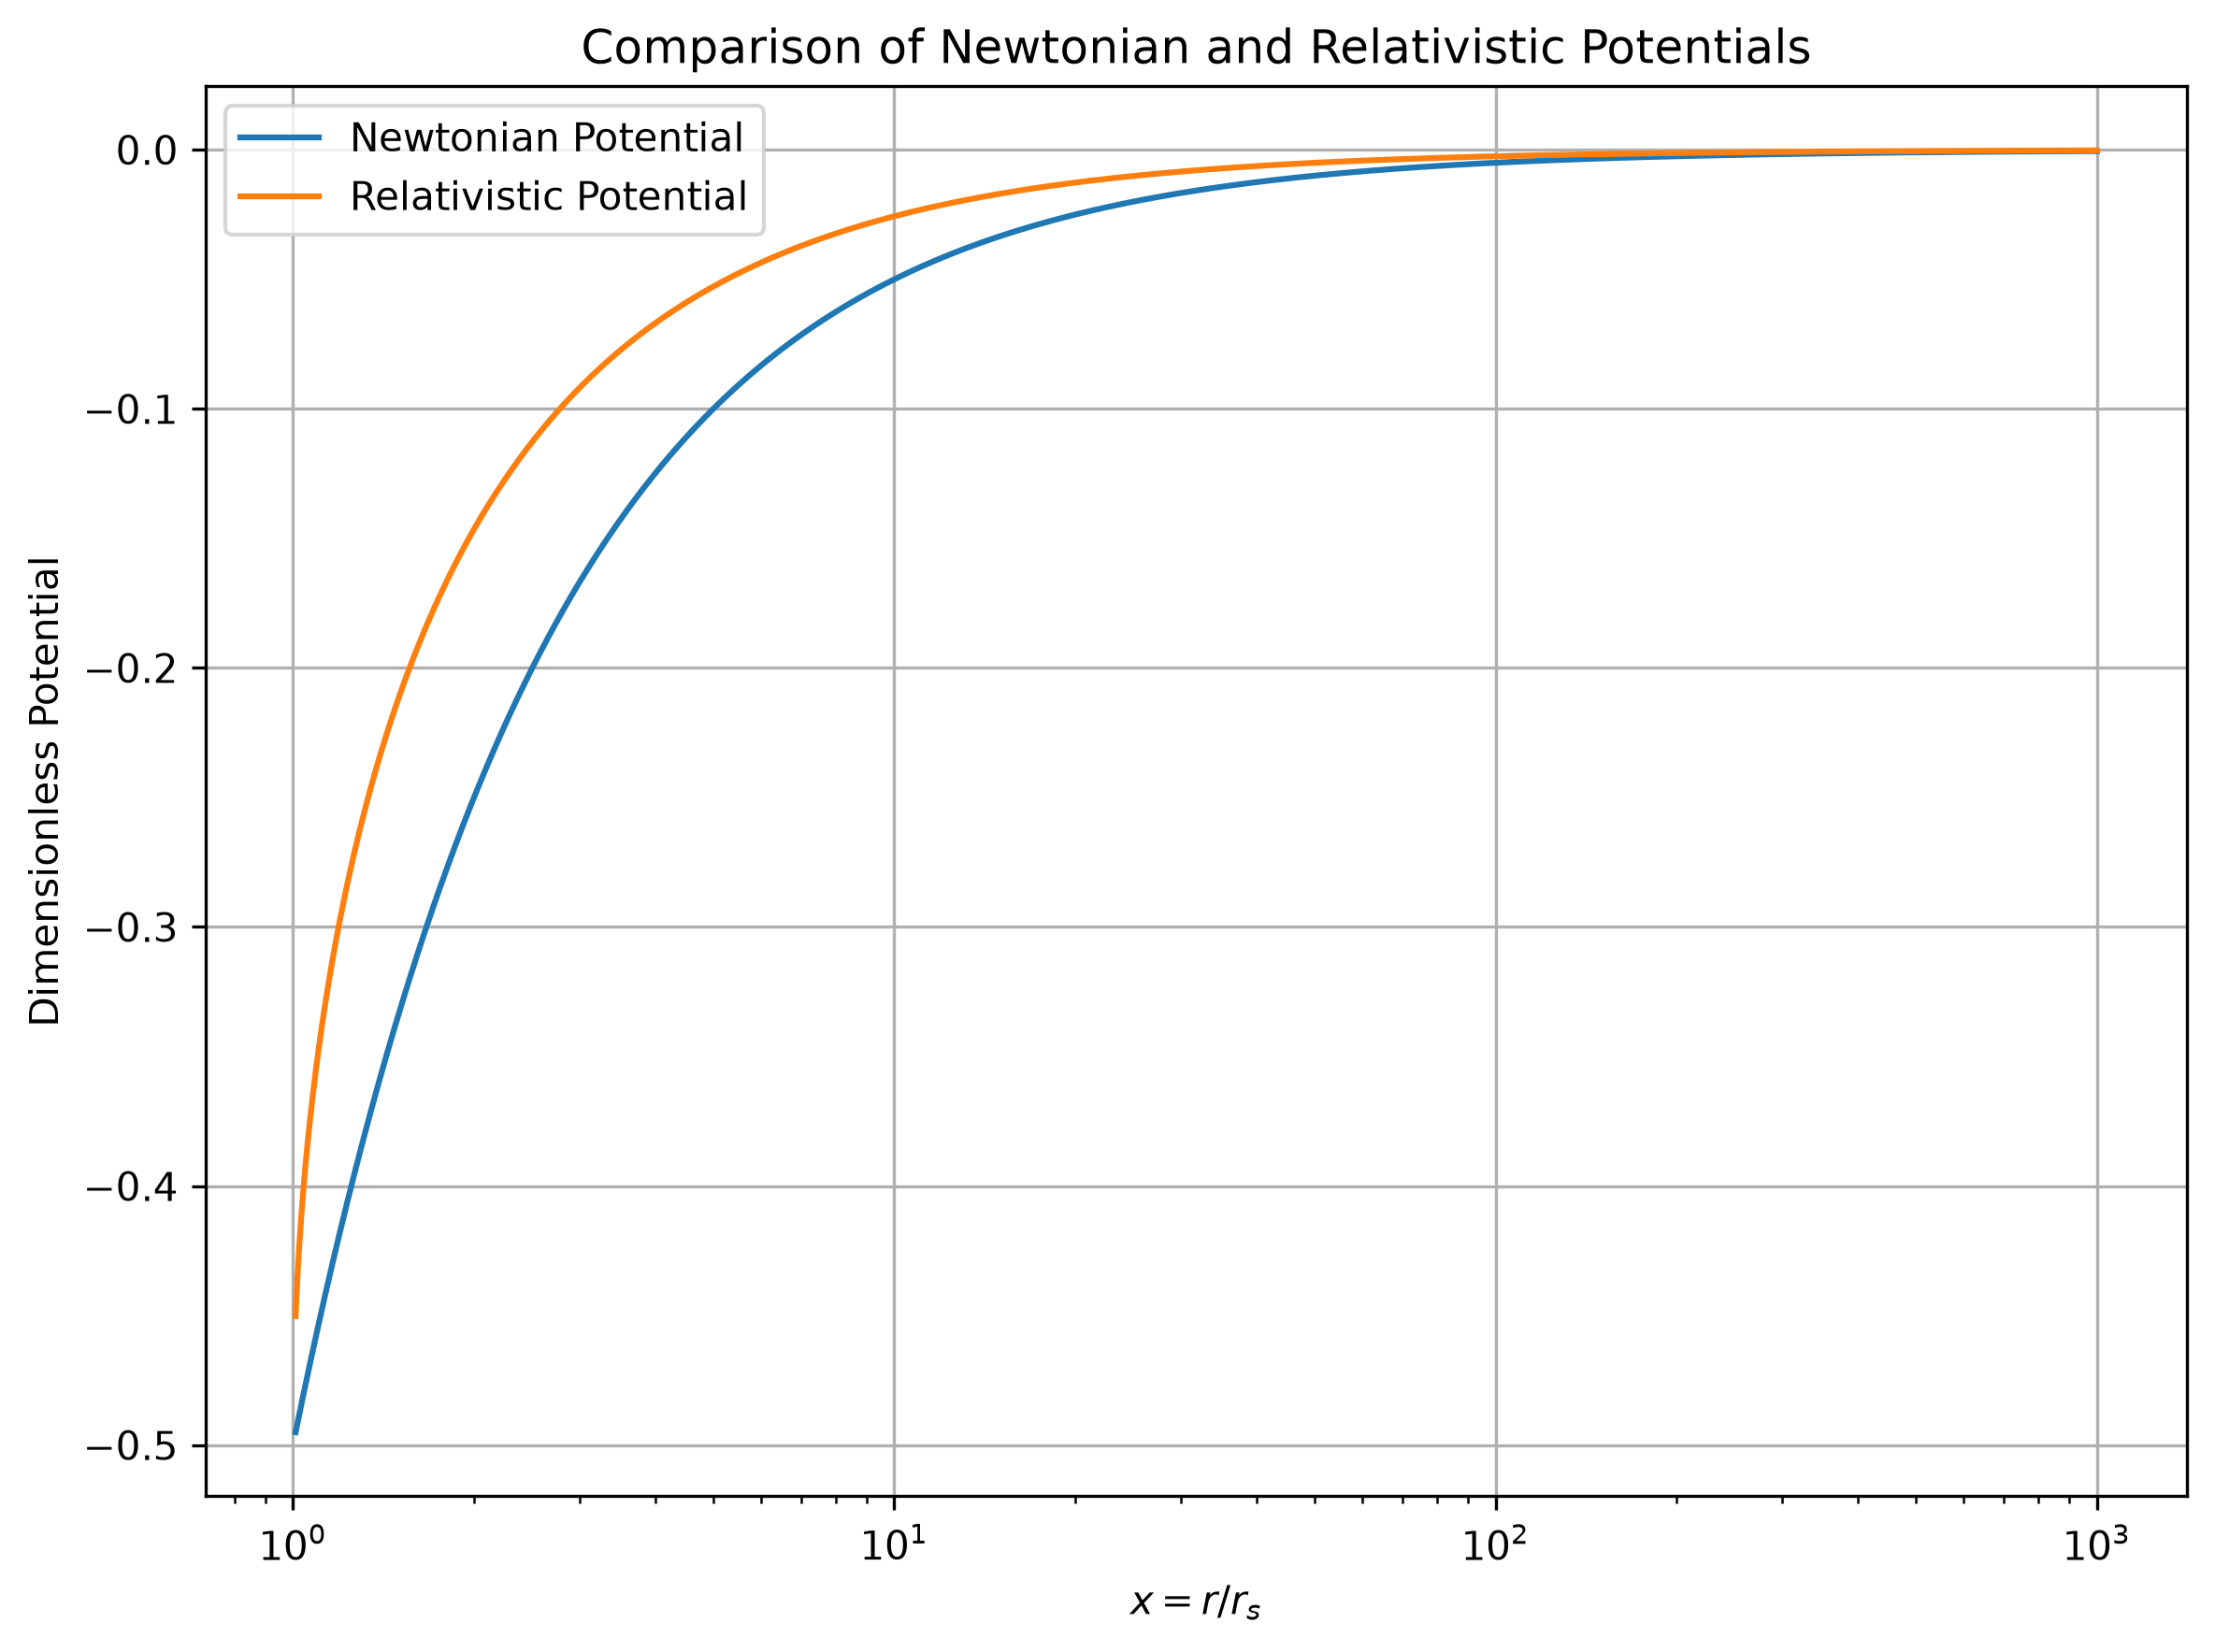
\includegraphics[width=0.85\textwidth]{../04_Graphs_and_Figures/potential_comparison.png}
\caption{Comparison of machine learning predictions with the analytical relativistic potential. The figure illustrates the ability of different models to reproduce the theoretical relationship.}
\label{fig:potential_comparison}
\end{figure}

A clear hierarchy in predictive performance is observed among the evaluated algorithms. Linear regression and polynomial regression exhibit comparatively large prediction errors, indicating that the dependence of the relativistic potential on the normalized radial coordinate is inherently nonlinear and cannot be represented adequately using low-order regression models.

The neural network substantially improves the approximation accuracy, achieving an $R^2$ value exceeding 0.98 while simultaneously reducing both the MAE and RMSE. This demonstrates its ability to learn the nonlinear structure of the generated physical dataset with high fidelity.

Among all evaluated models, random forest regression provides the highest predictive accuracy, yielding an almost perfect coefficient of determination ($R^2 \approx 0.999999$) together with extremely small prediction errors. The ensemble-based learning strategy enables the model to reproduce the analytical relativistic potential with remarkable precision throughout the investigated machine-learning domain. Such exceptional performance is expected because the training dataset is generated directly from a deterministic analytical function involving a single independent variable.

Overall, the results demonstrate that nonlinear machine learning methods provide substantially more accurate approximations of the relativistic potential than conventional regression techniques. They also illustrate the importance of selecting learning architectures capable of representing nonlinear physical relationships.

\subsubsection{Numerical Error Analysis Summary}\label{numerical-error-analysis-summary}

In addition to evaluating machine learning performance, the analytical formulation was investigated through numerical error analysis. The difference between the relativistic and Newtonian potentials is defined as

\[
\Delta\phi=\phi_{GR}-\phi_N
\]

The principal numerical results obtained from the computational analysis are summarized in Table~\ref{tab:error_summary}.

\begin{table}[H]
\centering
\caption{Summary of numerical error analysis results.}
\label{tab:error_summary}

\renewcommand{\arraystretch}{1.45}

\begin{tabular}{@{} l p{7cm} @{}}
\toprule
\textbf{Quantity} & \textbf{Value} \\
\midrule

Number of samples &
10,000 \\[2pt]

Numerical Analysis Domain &
$1.01 \leq x \leq 100$ \\[2pt]

Maximum deviation location &
$x=\frac{4}{3}$ \\[2pt]

Maximum deviation &
$\Delta\phi_{\max}=\frac{1}{8}$ \\[2pt]

Minimum relative error &
$9.950372\%$ \\[2pt]

Maximum relative error &
$99.949987\%$ (approaching $100\%$ as $x\rightarrow\infty$) \\

\bottomrule
\end{tabular}

\end{table}

The numerical investigation reveals that the minimum relative error occurs at the lower boundary of the computational domain ($x=1.01$), where the discrepancy between the relativistic and Newtonian potentials is approximately $9.95\%$. Throughout the investigated interval, neither the $5\%$ nor the $1\%$ relative-error thresholds are attained.

As the normalized radial coordinate increases, the relative error rises monotonically and approaches approximately $100\%$. This asymptotic behaviour originates from the fundamentally different mathematical forms of the relativistic and Newtonian potential functions. These results quantitatively illustrate the limitations of the Newtonian approximation within the adopted dimensionless formulation and provide a computational characterization of the transition between relativistic and classical gravitational descriptions.

\subsection{Prediction Analysis}\label{prediction-analysis}

To further assess the predictive capability of the evaluated machine learning algorithms, the model outputs were compared directly with the analytical relativistic potential generated from the theoretical formulation. Such comparisons provide a visual assessment of how accurately each learning algorithm reproduces the underlying physical relationship in addition to the numerical performance metrics presented previously.

The prediction curves illustrate the agreement between the normalized radial coordinate ($x$) and the corresponding relativistic potential $\phi_{GR}(x)$ across the investigated machine-learning domain.

The linear and polynomial regression models exhibit noticeable deviations from the analytical solution, particularly in regions where the potential varies nonlinearly. This behaviour reflects the limited representational capacity of these relatively simple regression techniques when applied to nonlinear physical systems.

The neural network produces a substantially improved approximation, closely following the analytical solution over the entire computational domain. Its ability to learn complex nonlinear mappings enables the model to reproduce the variation of the relativistic potential with considerably greater accuracy than conventional regression approaches.

Among the evaluated models, random forest regression provides the closest agreement with the analytical solution. The predicted values remain nearly indistinguishable from the theoretical curve throughout the investigated range, demonstrating that ensemble learning methods can effectively approximate deterministic nonlinear physical relationships when trained using sufficiently representative datasets.

The prediction capability of the random forest model is illustrated in Figure~\ref{fig:random_forest_prediction}.

\begin{figure}[H]
\centering
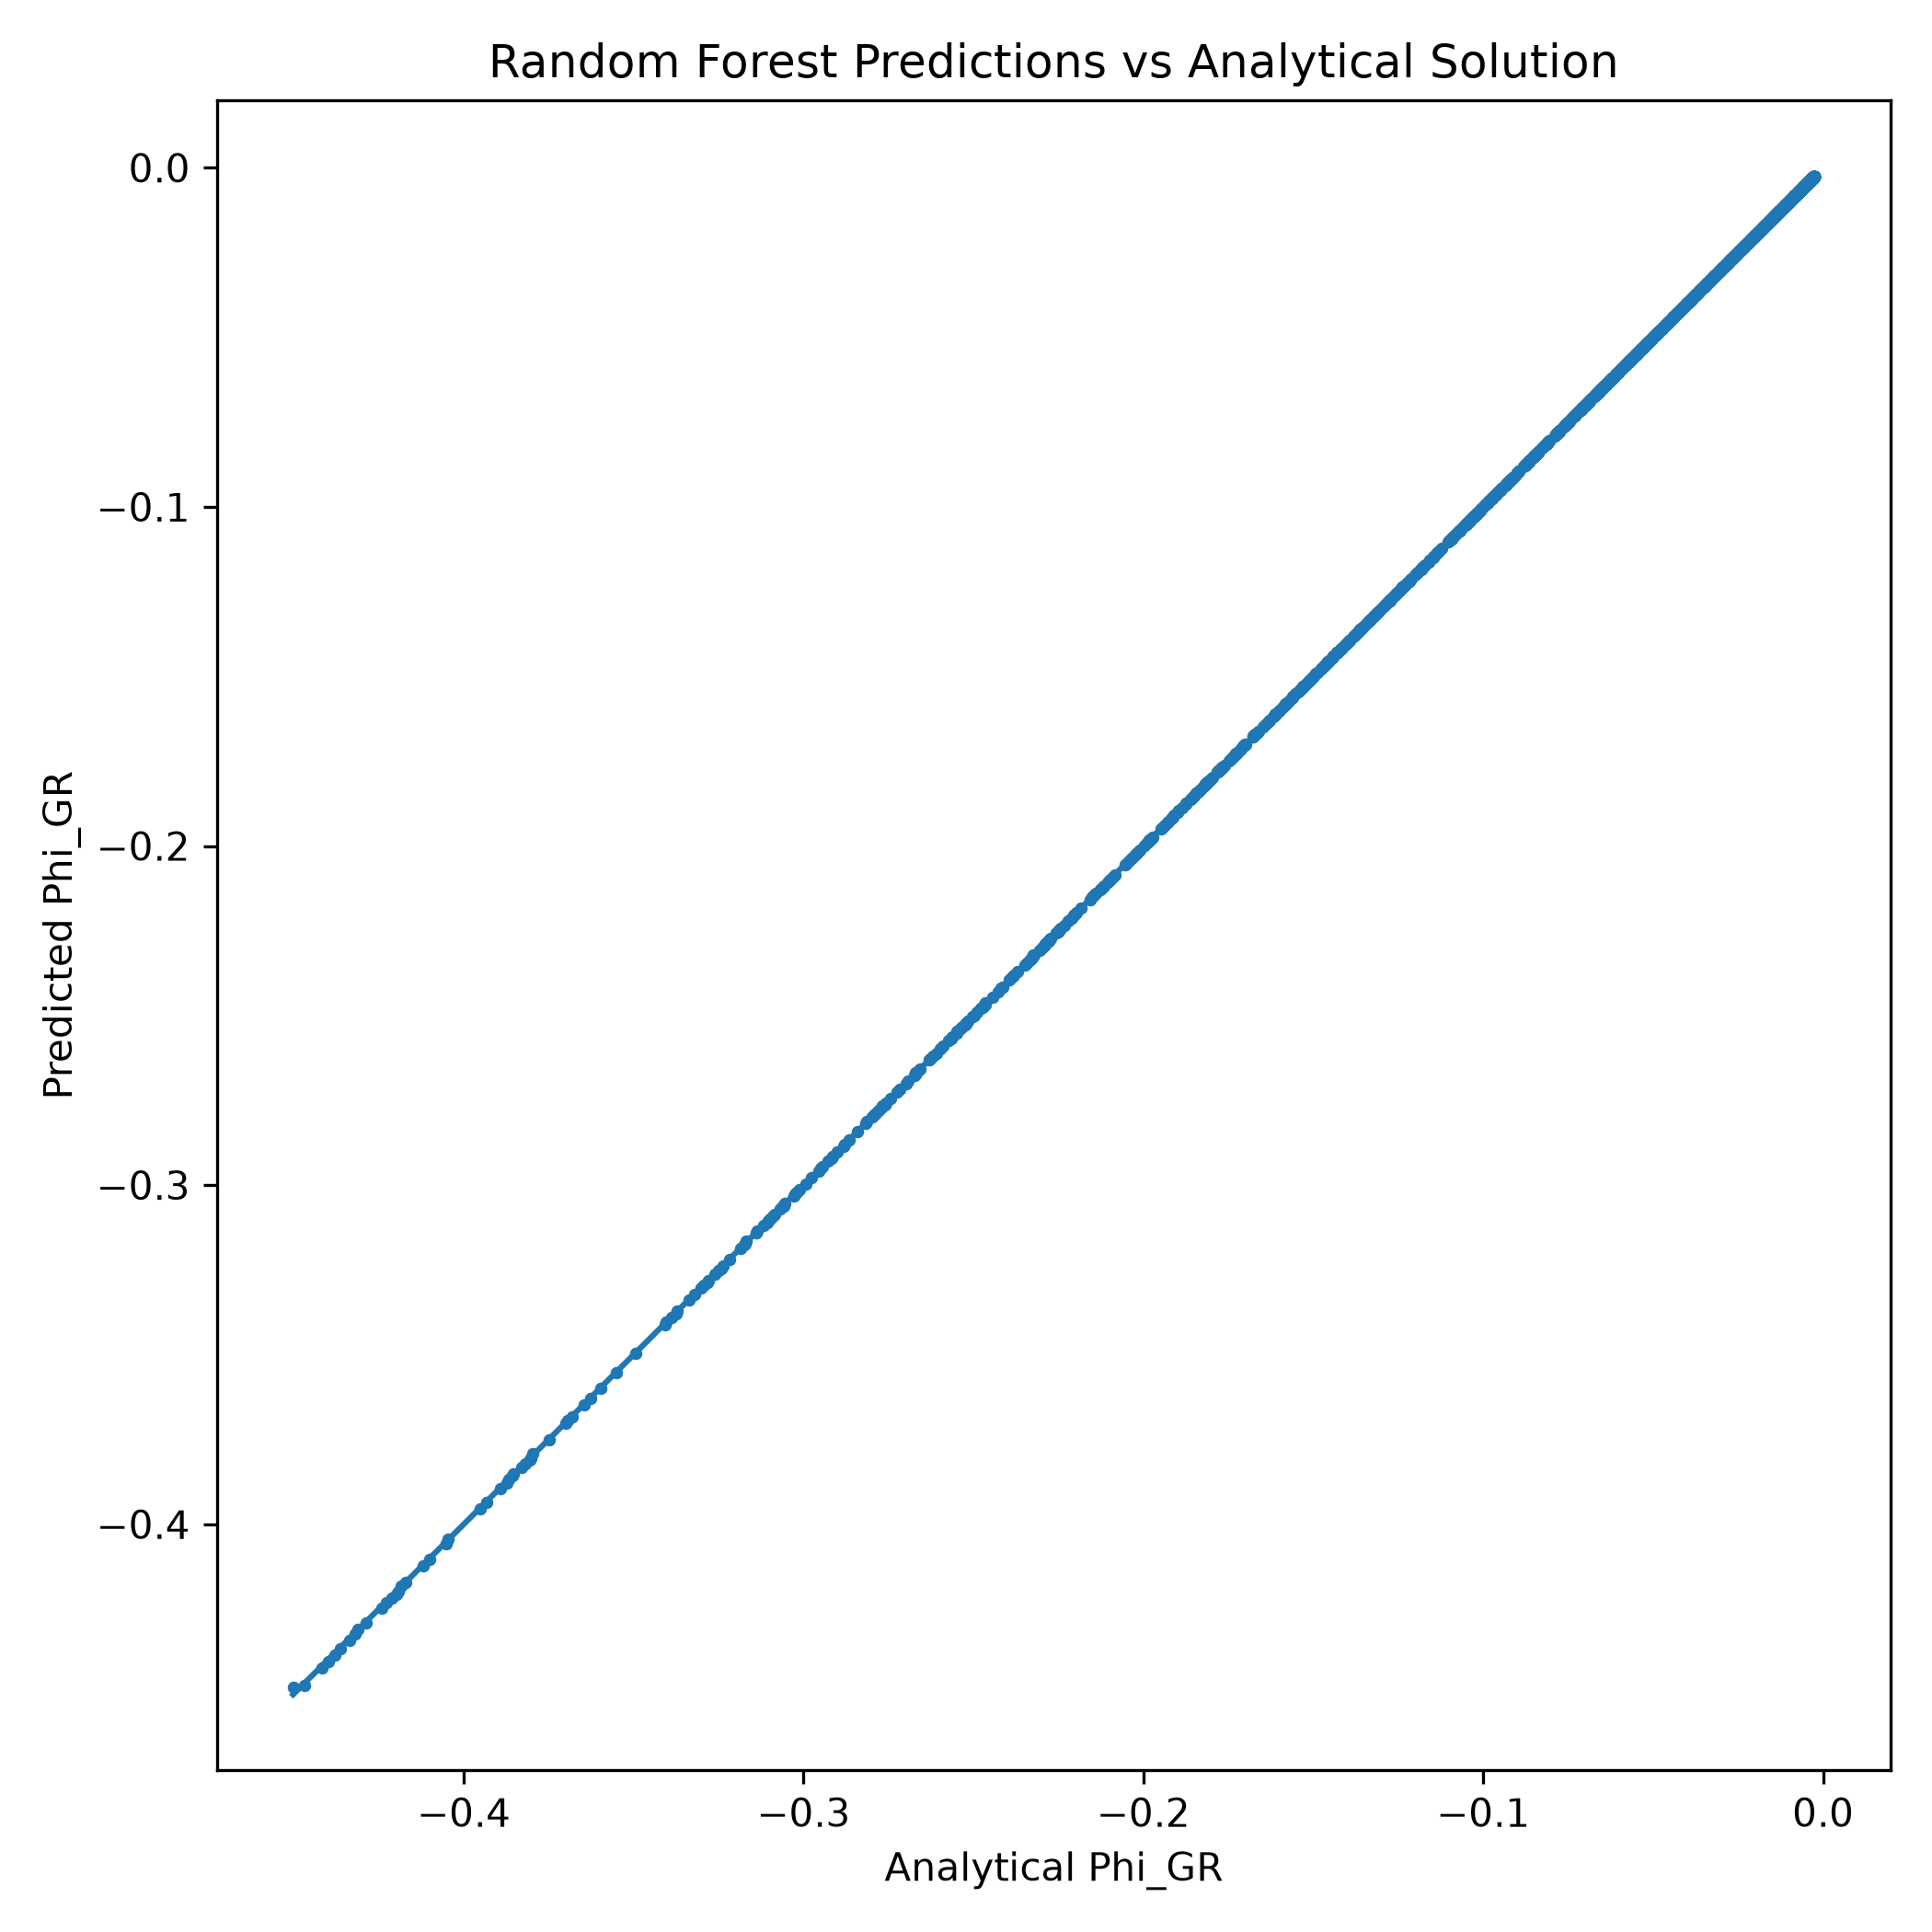
\includegraphics[width=0.85\textwidth]{../04_Graphs_and_Figures/random_forest_prediction.png}
\caption{Random forest regression predictions compared with the analytical relativistic potential over the machine-learning dataset range.}
\label{fig:random_forest_prediction}
\end{figure}

The prediction analysis supports the conclusions obtained from the quantitative performance metrics. Machine learning models possessing greater nonlinear representational capacity consistently provide more accurate approximations of the relativistic potential than simpler regression-based methods.

It should be emphasized, however, that the objective of the present investigation is not to replace the underlying physical model with a purely data-driven alternative. Since the training data are generated directly from the analytical relativistic potential, the machine learning algorithms function as computational surrogate models rather than independent methods for discovering physical laws. Their performance therefore reflects the ability to reproduce an established analytical relationship efficiently while preserving the essential characteristics of the underlying gravitational model.

\subsection{Residual Analysis}\label{residual-analysis}

To obtain a more detailed assessment of prediction accuracy, the performance of the machine learning models was further examined through residual analysis. Unlike global performance metrics such as MAE and RMSE, residual analysis provides information about the distribution of prediction errors throughout the computational domain and helps identify systematic deviations between the analytical model and its machine learning approximation.

The residual is defined as the difference between the analytical relativistic potential and the corresponding machine learning prediction:

\[
\mathrm{Residual}=\phi_{GR}(x)-\hat{\phi}_{GR}(x)
\]

where:

\begin{itemize}
\tightlist
\item
$\phi_{GR}(x)$ represents the analytical relativistic potential.
\item
$\hat{\phi}_{GR}(x)$ represents the machine learning prediction.
\end{itemize}

Residual analysis complements conventional regression metrics by revealing how prediction errors are distributed over the input domain. A model exhibiting small, randomly distributed residuals generally indicates that the underlying physical relationship has been captured successfully, whereas systematic residual patterns may suggest deficiencies in the model structure or approximation capability.

The linear and polynomial regression models exhibit comparatively larger residuals, particularly in regions where the relativistic potential varies nonlinearly. These deviations are consistent with the limited flexibility of simple regression models and further demonstrate that low-order mathematical approximations are insufficient for accurately representing the nonlinear behaviour of the relativistic potential.

In contrast, the neural network and random forest models produce substantially smaller residuals across the investigated domain. The reduction in prediction error confirms their ability to capture the nonlinear dependence of the relativistic potential on the normalized radial coordinate with significantly greater accuracy.

Residual analysis also provides insight into the local reliability of machine learning predictions. Regions exhibiting comparatively larger residuals identify portions of the parameter space where approximation becomes more challenging and therefore provide useful information regarding the limitations of each learning algorithm.

Consequently, residual analysis complements the global performance metrics presented previously by providing a more comprehensive evaluation of how effectively each machine learning model reproduces the analytical relativistic potential.

The residual distribution obtained from the machine learning predictions is illustrated in Figure~\ref{fig:residual_plot}.

\begin{figure}[H]
\centering
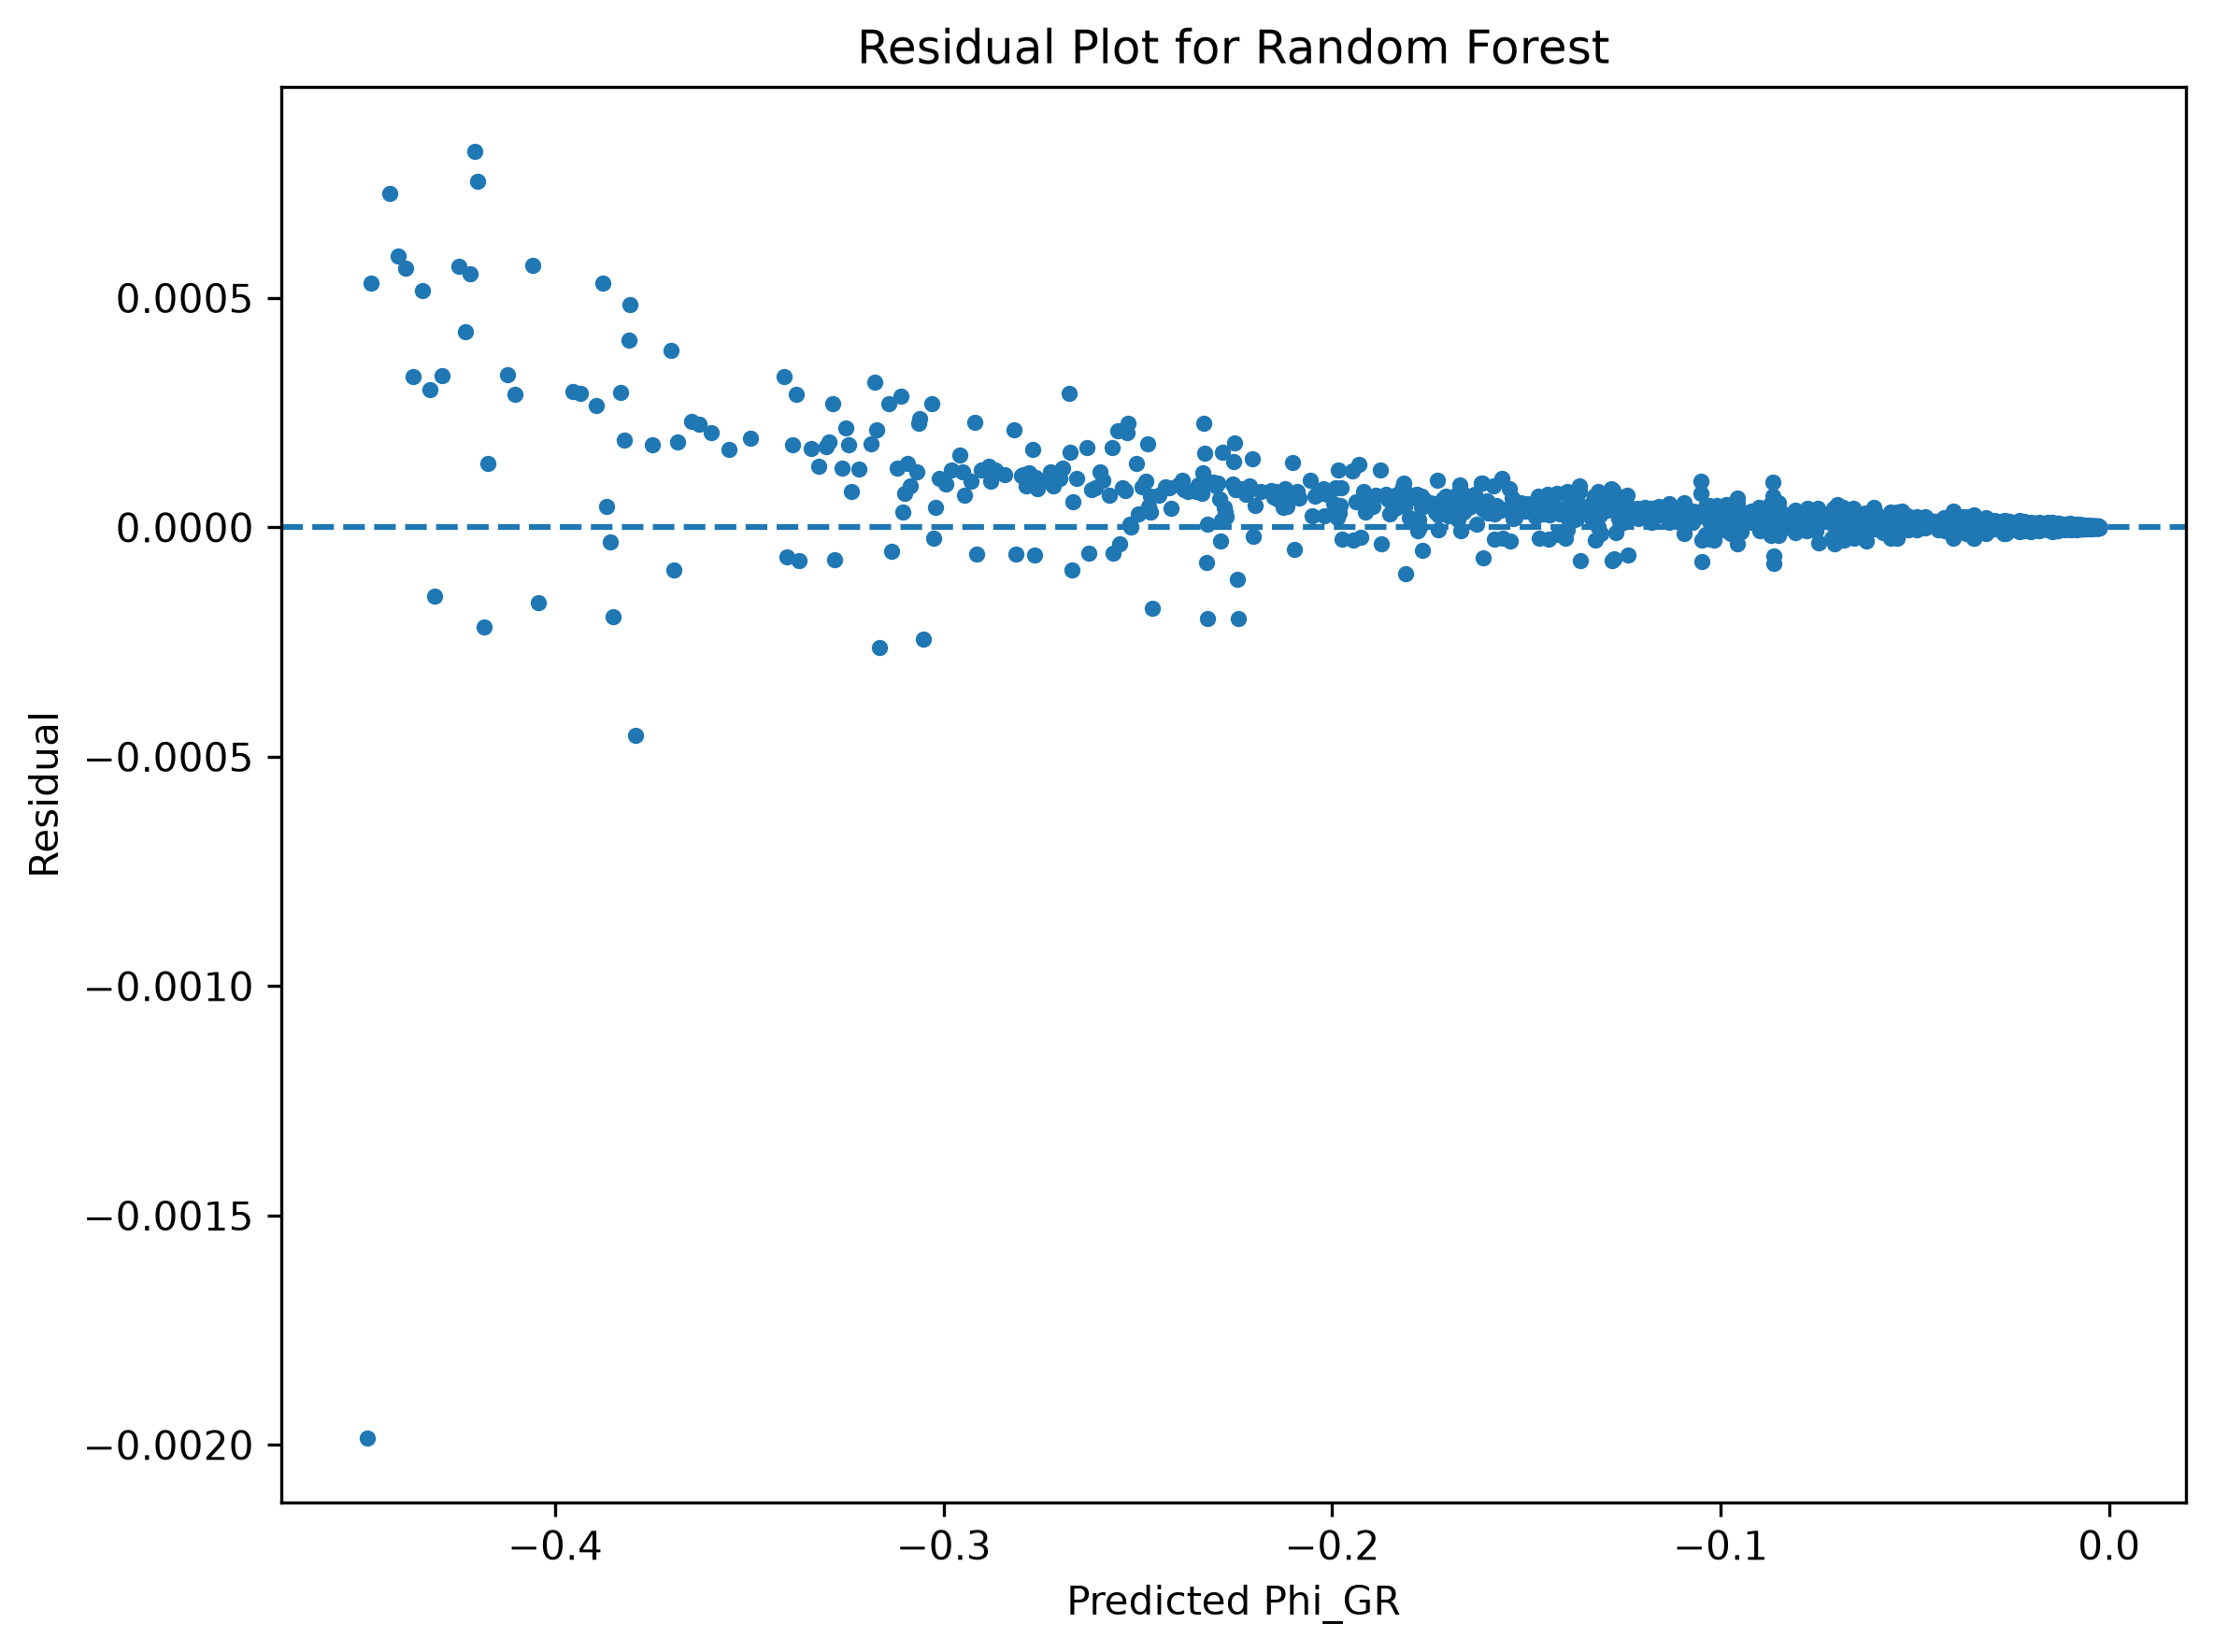
\includegraphics[width=0.85\textwidth]{../04_Graphs_and_Figures/residual_plot.png}
\caption{Residual distribution obtained from machine learning predictions, showing the difference between analytical and predicted relativistic potential values.}
\label{fig:residual_plot}
\end{figure}

\subsection{Feature Importance Results}\label{feature-importance-results}

In addition to predictive accuracy, the interpretability of machine learning models is an important consideration in scientific applications. Feature importance analysis was therefore performed to examine the contribution of the input variable to the prediction process and to verify that the learned relationship remains consistent with the underlying physical formulation.

The present dataset contains a single physical input parameter,

\[
x=\frac{r}{r_s},
\]

which represents the normalized radial coordinate. Since the relativistic potential is explicitly defined as a function of this variable, the prediction produced by each machine learning model is entirely determined by the variation of $x$.

For tree-based algorithms such as random forest regression, feature importance is evaluated by measuring the contribution of each input variable to the reduction of prediction uncertainty throughout the ensemble of decision trees. Although the present study involves only a single input feature, this analysis provides an additional verification that the model attributes its predictive capability to the physically meaningful variable governing the analytical formulation.

The feature importance results confirm that the normalized radial coordinate constitutes the complete source of predictive information within the generated dataset. This observation is fully consistent with the mathematical model, in which the relativistic potential depends solely on the dimensionless radial coordinate.

Although feature importance analysis is more informative for datasets containing multiple physical variables, its inclusion here establishes a transparent framework for interpreting machine learning models within a scientific context. Such interpretability analyses become increasingly valuable when extending the present methodology to more complex gravitational systems involving additional physical parameters.

Consequently, the combination of predictive performance evaluation and model interpretability provides a more comprehensive assessment of the applicability of machine learning techniques to computational physics problems.

The contribution of the input variable to the prediction process is illustrated in Figure~\ref{fig:feature_importance}.

\begin{figure}[H]
\centering
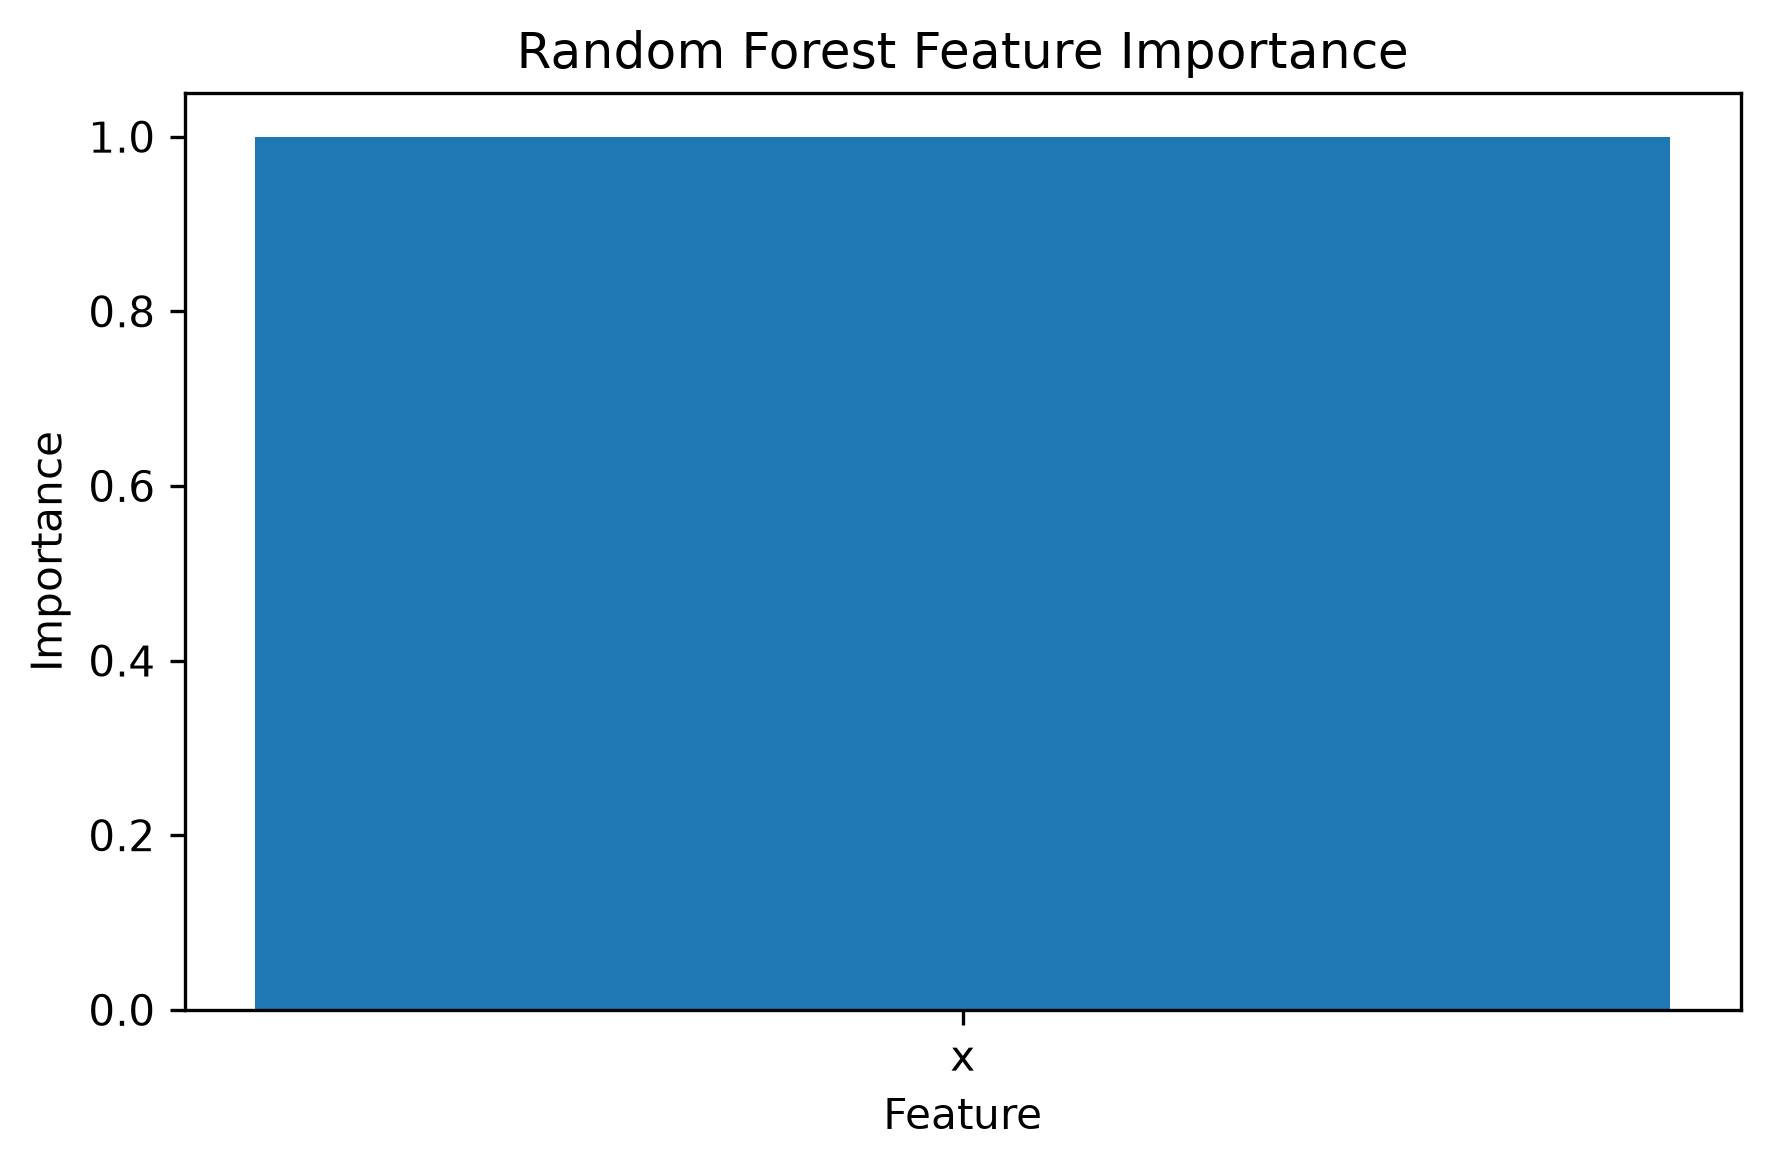
\includegraphics[width=0.85\textwidth]{../04_Graphs_and_Figures/feature_importance.png}
\caption{Feature importance obtained from the random forest model. The normalized radial coordinate $x$ is the sole input feature and therefore accounts for the complete predictive contribution.}
\label{fig:feature_importance}
\end{figure}

\section{Discussion}\label{discussion}

\subsection{Physics Interpretation}\label{physics-interpretation}

The analytical and computational results provide a quantitative
understanding of the relationship between classical and relativistic
descriptions of gravitational behaviour.

The error analysis demonstrates that the Newtonian approximation can
successfully reproduce the qualitative characteristics of the
relativistic model in the weak-field regime. However, the quantitative
difference between the two descriptions becomes increasingly significant
as the gravitational field strength increases. This behaviour is
consistent with the expected domain of validity of classical
gravitational approximations, where relativistic corrections become
important only beyond the weak-field limit.

The increasing deviation between the Newtonian and relativistic models
in stronger-field regions highlights the limitations of extending
classical approximations beyond their applicable range. The transition
between relativistic and Newtonian behaviour does not occur at a sharp
boundary; instead, it represents a continuous change that can be
systematically quantified using the relative error function.

The computational framework developed in this study allows this
transition to be investigated by identifying the regions in which the
Newtonian approximation satisfies specific accuracy requirements. This
provides a measurable interpretation of the validity range of the
classical approximation within the considered relativistic potential
model.

The results further demonstrate the importance of combining analytical
and computational methods in the investigation of physical systems.
While the mathematical formulation establishes the theoretical basis of
the model, numerical analysis enables detailed examination of its
behaviour across different gravitational regimes.

This integration of analytical physics and computational techniques
provides the foundation for the machine learning analysis presented in
this work, where data-driven methods are evaluated as computational
approximations of the established physical relationship.

\subsection{Machine Learning Interpretation}\label{machine-learning-interpretation}

The machine learning results demonstrate the capability of data-driven
methods to approximate the behaviour of a nonlinear physical system
generated from an analytical gravitational model.

The comparison between different algorithms shows that model selection
has a significant influence on approximation performance. Simpler
methods, such as linear regression, provide an important baseline but
are limited in their ability to represent the nonlinear structure of the
relativistic potential.

The improved performance of neural networks and random forest regression
demonstrates that flexible machine learning architectures can effectively
capture complex relationships present within physically generated
datasets. These models successfully reconstruct the numerical behaviour
of the relativistic potential without requiring repeated evaluation of
the original analytical expression during prediction.

However, the purpose of machine learning in this study is not to replace
the underlying physical formulation. Since the training data is generated
directly from the analytical relativistic potential, the machine learning
models are evaluated as approximation techniques rather than independent
methods for discovering the governing physical law.

This distinction is important in scientific machine learning, where
predictive accuracy must be considered together with physical
consistency and interpretability. The present study provides a controlled
benchmark in which machine learning models can be compared against an
exact theoretical solution, allowing their approximation capability to be
evaluated objectively.

The framework demonstrates the potential of machine learning models as
surrogate computational tools for nonlinear physical systems. Such
approaches may become particularly useful in situations where repeated
evaluation of complex models becomes computationally expensive while the
underlying physical constraints remain well established.

This concept is consistent with the broader development of scientific
machine learning, where data-driven methods are combined with physical
knowledge to improve computational efficiency and modelling capability
\cite{karniadakis2021}.

\subsection{Limitations and Future Extensions}\label{limitations-and-future-extensions}

Although the results demonstrate the effectiveness of machine learning
methods for approximating the relativistic potential, several
limitations of the present framework should be acknowledged.

The current dataset is generated from a deterministic analytical model
with a single independent variable. This controlled setup allows a clear
evaluation of machine learning performance; however, realistic physical
systems generally involve multiple parameters, complex boundary
conditions, observational uncertainties, and interactions between
different physical processes.

Furthermore, the high prediction accuracy obtained by some models is
dependent on the quality, distribution, and range of the generated
dataset. A model trained within a specific parameter range may not
generalize accurately beyond that range without additional training
data or appropriate physical constraints.

Future extensions of this work may include incorporating additional
physical parameters, investigating more complex gravitational systems,
and evaluating machine learning performance using independently generated
numerical simulations or observational datasets.

Another important direction is the development of physics-informed
machine learning approaches, where governing physical principles are
directly incorporated into the learning process. Such methods provide a
framework for combining the flexibility of machine learning with the
reliability of established physical laws \cite{karniadakis2021}.

These extensions would allow the methodology developed in this study to
move beyond approximation of a single theoretical relationship toward
more complex scientific modelling problems where analytical solutions
may be unavailable or computationally expensive.

The present work represents a controlled demonstration of how
analytical physics models, numerical analysis, and machine learning
techniques can be integrated within a unified computational framework.
Although the current investigation focuses on a single relativistic
potential, the proposed methodology provides a foundation for applying
similar approaches to broader problems in computational physics.

\section{Conclusion}

This study presented a combined analytical, numerical, and machine
learning framework for investigating a static relativistic gravitational
potential and its relationship with the Newtonian approximation.

The theoretical analysis established the mathematical formulation of the
relativistic potential and provided a quantitative comparison with the
classical model through relative error analysis. The results
demonstrated that although the Newtonian approximation reproduces the
general inverse-distance behavior of the relativistic model, a
systematic quantitative difference remains due to the different
asymptotic behavior of the two formulations.

The numerical analysis allowed the deviation between the two models to
be investigated across different gravitational regimes. By evaluating
the relative error over the selected domain, the study identified the
limitations of the Newtonian approximation under the considered
formulation and demonstrated how computational methods can provide
measurable criteria for approximation validity.

The machine learning component further explored the ability of
data-driven models to approximate the relativistic potential from
generated physical data. The comparison between linear regression,
polynomial regression, neural networks, and random forest regression
showed that models with greater capability to represent nonlinear
relationships achieved improved prediction performance.

However, the machine learning models were treated as computational
approximations rather than replacements for the underlying physical
formulation. The analytical model remains the source of the physical
relationship, while machine learning provides an alternative method for
efficient numerical representation.

Overall, this study demonstrates the potential of integrating theoretical
physics, numerical computation, and machine learning for studying
nonlinear scientific systems. The developed framework provides a
foundation for future extensions involving more complex gravitational
models, additional physical parameters, and physics-informed machine
learning approaches.

\section{Data and Code Availability}

The complete source code, datasets, machine learning scripts, generated figures, and supplementary materials associated with this study are publicly available at:

\url{https://github.com/Dev-Aayush-Kumar/computational-gravity-ml}

This repository contains all computational workflows used to generate the numerical results, machine learning models, datasets, and visualizations presented in this paper.

\section{Acknowledgements}

I would like to express my deepest gratitude to my parents for their unwavering support and my brother for keeping me amused throughout this research project and my broader academic journey. Their encouragement, patience, and belief in my abilities have been a constant source of motivation, especially during challenging periods. I am grateful for the opportunities, resources, and supportive environment they provided, which enabled me to pursue this study alongside my academic studies and future educational goals.

I would also like to thank a school friend whose own research publication motivated me to begin this journey. Seeing a fellow student undertake independent research helped me realize that such goals were achievable and encouraged me to pursue my own AI interests with greater confidence and determination.

Finally, I would like to express my profound appreciation to a very special individual whose influence on my personal and academic growth has been immeasurable. At a time when I often underestimated my own potential and struggled with distractions, self-doubt, and uncertainty about my direction, this person consistently encouraged me to aim higher and take my ambitions seriously.

More importantly, this individual demonstrated a level of belief in my abilities that often exceeded my own. Through encouragement, honest conversations, constructive advice, and unwavering support, I gradually began to recognize possibilities within myself that I had previously overlooked. The confidence, discipline, and sense of purpose developed during this period played an important role in enabling me to undertake projects such as the present work.

The research presented in this paper is the result of many months of study, persistence, and effort. However, much of the determination required to begin and continue this journey was strengthened by the support and encouragement received from this individual. Beyond the completion of this project, the influence has extended to broader academic aspirations, personal development, and the pursuit of goals that once seemed beyond reach.

Some contributions to a person's growth cannot be measured through equations, datasets, or performance metrics. Nevertheless, they can leave a lasting impact. For that reason, I offer my sincere gratitude and appreciation for the encouragement, faith, and motivation that helped make this study possible.

\newpage
\bibliographystyle{ieeetr}
\bibliography{references}

\end{document}
